% Preamble
\pdfminorversion=4
\documentclass[aspectratio=169]{beamer}
%\usepackage{multimedia} % for videos
\usepackage{movie15}
\usepackage{bm} % for bold math (for tensors)
\usepackage{layout} % put command \layout{} onto an empty frame to see margin lengths
\usepackage{adjustbox}
\usepackage{lipsum}
\usepackage{pdfpages}
\usepackage{hyperref} % for hyperlinks
\usepackage{ulem} % for underline, etc.
\usepackage{layouts}
\usepackage{amsmath, nccmath}
\usepackage{algorithm}
\usepackage{algpseudocode}
\usepackage{overpic}
\setbeamertemplate{bibliography item}{\insertbiblabel} %% Remove book symbol from references and add number
\usepackage[style=ieee,backend=bibtex,citetracker=true]{biblatex} %footnote refs
\addbibresource{refs.bib}

%for collabortation/commenting
\newcommand{\Doug}[1]{{\color{blue}#1}}
\newcommand{\Pierre}[1]{{\color{red}PIERRE:#1}}

% ----- beamer settings -----
% {{{

% define some colors/shades
\definecolor{DarkGreen}{rgb}{0.0,100/128,0.0}
\definecolor{Redd}{rgb}{1.0,0.0,0.0}
\definecolor{Lavender}{HTML}{4D00FF}
\definecolor{lightblue}{HTML}{66A3D2}
\definecolor{darkblue}{HTML}{0B61A4}
\definecolor{lightorange}{HTML}{FF8E0B}
\definecolor{darkorange}{HTML}{D45500}
\definecolor{paleorange}{HTML}{FFDEB3}
\definecolor{FigGreen}{HTML}{009B72}
\definecolor{FigOrange}{HTML}{E36414}
\definecolor{FigPurple}{HTML}{985277}
%\definecolor{FigDarkGreen}{HTML}{}

% set color for hyperlinks
\hypersetup{colorlinks, linkcolor=darkgray, citecolor=darkgray, urlcolor=darkgray}

% set theme
\usetheme{boxes}
\usefonttheme[onlymath]{serif}

% set beamer theme colors, etc.
\setbeamercolor{frametitle}{fg=black}

% customize blocks
\setbeamertemplate{blocks}[rounded][shadow=false]
\setbeamercolor{block title}{fg=white, bg=darkblue}
\setbeamercolor{block body}{fg=black, bg=lightblue}

% customize enumerate and item, including color and spacing
\setbeamercolor*{item}{fg=darkblue}
\setbeamercolor*{enumerate item}{fg=black}
\setbeamercolor*{enumerate subitem}{fg=black}
\setbeamercolor*{enumerate subsubitem}{fg=black}
\setbeamertemplate{itemize subitem}{$-$}
\setlength{\leftmarginii}{10pt}
\newlength\origleftmargini
\setlength\origleftmargini\leftmargini

% customize footer
\setbeamercolor{footline}{fg=gray}
\setbeamertemplate{navigation symbols}{} % get rid of navigation bar

% add page numbers to footer
\makeatletter
\setbeamertemplate{footline}{
    \leavevmode%
    \hbox{%
    \begin{beamercolorbox}[wd=0.5\paperwidth,ht=2.25ex,dp=1ex,left,leftskip=1ex]{}
    \end{beamercolorbox}
    \begin{beamercolorbox}[wd=0.5\paperwidth,ht=2.25ex,dp=1ex,right,rightskip=2ex]{}
      \large \insertframenumber % page number only
      % \insertframenumber/\inserttotalframenumber % page number/total pages
    \end{beamercolorbox}
    }\vskip0pt
}

% See https://tex.stackexchange.com/a/396754/28146
\newbibmacro*{hypercite}{%
  \renewcommand{\@makefntext}[1]{\noindent\normalfont##1}%
  \footnotetext{%
    \blxmkbibnote{foot}{%
    \printtext[labelnumberwidth]{%
      \printfield{prefixnumber}%
      \printfield{labelnumber}}%
    \addspace
    \printnames[][1-1]{author}
    \setunit{\addcomma\addspace}
    \printfield{journaltitle}
    \setunit{\addcomma\addspace}
    \printfield{year}
    }}}

\DeclareCiteCommand{\hypercite}%
  {\usebibmacro{cite:init}}
  {\usebibmacro{hypercite}}
  {}
  {\usebibmacro{cite:dump}}

% Redefine the \footcite command to use the reference number
\renewcommand{\footcite}[1]{\cite{#1}\hypercite{#1}}

\newbox\@backgroundblock
\newenvironment{backgroundblock}[2]{%
  \global\setbox\@backgroundblock=\vbox\bgroup%
    \unvbox\@backgroundblock%
    \vbox to0pt\bgroup\vskip#2\hbox to0pt\bgroup\hskip#1\relax%
}{\egroup\egroup\egroup}
\addtobeamertemplate{background}{\box\@backgroundblock}{}

\makeatother
% }}}

% ----- tikz ----- (for drawing)
% {{{
\usepackage{tikz}
\usetikzlibrary{shapes,positioning,arrows,backgrounds,fit,chains}

% tikz define invisible: 
% http://tex.stackexchange.com/questions/55806/mindmap-tikzpicture-in-beamer-reveal-step-by-step/55849#55849
\tikzset{
  invisible/.style={opacity=0.2},
  visible on/.style={alt=#1{}{invisible}},
  alt/.code args={<#1>#2#3}{%
    \alt<#1>{\pgfkeysalso{#2}}{\pgfkeysalso{#3}} % \pgfkeysalso doesn't change the path
  },
  startstop/.style={
    rectangle, 
    rounded corners,
    minimum width=3cm, 
    minimum height=1cm,
    align=center, 
    draw=black, 
    fill=red!30
    },
  process/.style={
    rectangle, 
    minimum width=3cm, 
    minimum height=1cm, 
    align=center, 
    draw=black, 
    fill=blue!30
    },
  decision/.style={
    rectangle, 
    minimum width=3cm, 
    minimum height=1cm, align=center, 
    draw=black, 
    fill=green!30
    },
  arrow/.style={thick,->,>=stealth},
  dec/.style={
    ellipse, 
    align=center, 
    draw=black, 
    fill=green!30
    },
}

\pgfdeclarelayer{bg}    % declare background layer
\pgfsetlayers{bg,main}  % set the order of the layers (main is the standard layer)

\newcommand{\highlighteq}[2]{ \tikz[baseline]{\node[fill=#1,rounded corners,anchor=base]{$\displaystyle \strut #2$};} }

\tikzset{onslide/.code args={<#1>#2}{%
  \only<#1>{\pgfkeysalso{#2}} % \pgfkeysalso doesn't change the path
}}

% }}}

% --- Notes on options for including movies ---
% {{{

% (1) movie15 package
%\usepackage{movie15}
% \includemovie[text={\includegraphics[width=5cm]{figs/lam_t0.pdf}}]{}{}{figs/lam.avi}
% Comments: 
%   * apparently depreciated (superceded by movie9), but seems to play movies fine
%   * (bad) Puts a pushpin icon over the video
%   * (good) Actually embeds the movie, so don't need to include a separate folder
%   * (bad) Puts black or white bars when playing movie with controls (changes size of
%     the movie to fit the controls into the frame).

% (2) movie9 package
% \usepackage{media9}
% Comments:
%   * Plays using a flash player. Doesn't work on Linux.

% (3) multimedia package
% \usepackage{multimedia}
% \movie[width=5cm, showcontrols]{\includegraphics[width=5cm]{figs/lam_t0.pdf}}{figs/lam.avi}
% Comments:
%   * (good) Seems like the best (but flawed) option for playing a movie in the frame
%   * (bad) Does not embed the movie. Need a separate videos folder.
%   * (bad) Puts black or white bars when playing movie with controls (changes size of
%     the movie to fit the controls into the frame).
%   * (aside) Appears that the backend of the player (same as movie15 pacakge) can be 
%     changed from gstreamer to vlc. Used apt-get install phonon-backend-vlc. Made bars
%     white, not black, which was a marginal improvement.
%     http://tex.stackexchange.com/questions/163089/okular-to-play-embedded-videos-in-beamer

% (4) Hyperlink
% \include{hyperref}
% \href{run:figs/lam.avi}{\includegraphics[width=5cm]{figs/lam_t0.pdf}}
% Comments:
%   * Runs an external viewer (like VLC)
%   * (good) Cross-platform compatible
%   * (bad) Means lots of clicking, and not very easy to move back and forth
%   * (bad) Does not embed the movie. Need a separate videos folder.
%   * (bad) Cannot set up a script to give arguments to external program (e.g. VLC)

% (5) pdfpc
% \href{run:figs/lam.avi?autostart&loop}{\includegraphics[width=5cm]{figs/lam_t0.pdf}}
% Comments:
%   * (neutral) Separate presentation platform. Has nice features.
%   * (bad) Has a slow "pre-rendering" feature.
%   * (bad) All tested videos end up very poor resolution.
%   * (good) Viewer does not re-size videos with ugly controls

% }}}

% ----- tips/tricks & custom definitions ----
% {{{

%% ** block title without a block **
\newcommand{\blocktitleinv}[1]{
  \begin{tikzpicture}
    \node[ fill, color=white, text=white, rounded corners, inner sep=4pt,
           align=center, minimum width=4cm, minimum height=\baselineskip
    ] 
    {\large #1\par};
  \end{tikzpicture}
}

%% ** block with no fill **
\newcommand{\blocknofill}[1]{
  \begin{tikzpicture}
    \node[ draw, color=blue, very thick, rounded corners, minimum width=4cm, minimum height=\baselineskip ] %fill, color=white, text=white, rounded corners, inner sep=4pt,
   %        align=center, 
   % ] 
    {\large #1\par};
  \end{tikzpicture}
}

%% ** block title without a block **
\newcommand{\blocktitlesmall}[1]{
  \begin{tikzpicture}
    \node[ fill, color=darkblue, text=white, rounded corners, inner sep=4pt,
           align=center, minimum width=4cm, minimum height=\baselineskip
    ] 
    {\normalsize #1\par};
  \end{tikzpicture}
}

%% ** block title without a block **
\newcommand{\blocktitle}[1]{
  \begin{tikzpicture}
    \node[ fill, color=darkblue, text=white, rounded corners, inner sep=4pt,
           align=center, minimum width=4cm, minimum height=\baselineskip
    ] 
    {\large #1\par};
  \end{tikzpicture}
}

%% ** block title without a block green **
\newcommand{\blocktitlegreen}[1]{
  \begin{tikzpicture}
    \node[ fill, color=DarkGreen, text=black, rounded corners, inner sep=4pt,
           align=center, minimum width=4cm, minimum height=\baselineskip
    ] 
    {\LARGE #1\par};
  \end{tikzpicture}
}

%% ** block title without a block blue **
\newcommand{\blocktitleblue}[1]{
  \begin{tikzpicture}
    \node[ fill, color=blue, text=white, rounded corners, inner sep=4pt,
           align=center, minimum width=4cm, minimum height=\baselineskip
    ] 
    {\LARGE #1\par};
  \end{tikzpicture}
}

\newcommand\Wider[2][3em]{%
\makebox[\linewidth][c]{%
  \begin{minipage}{\dimexpr\textwidth+#1\relax}
  \raggedright#2
  \end{minipage}%
  }%
}

% ** columns **
%  \begin{columns}[T]
%    \begin{column}{0.45\textwidth}
%      Column 1: Theory
%    \end{column}
%    \begin{column}{0.45\textwidth}
%      Column 2: Experiment
%    \end{column}
%  \end{columns}

% ** make a figure bigger than the textwidth **
%\makebox[\textwidth][c]{\includegraphics[width=1.0\textwidth]{figs/immersion_precipitation_roll.pdf}}

% ** bulk commenting **
%\iffalse
%\fi

% ** Put citation in bottom middle **
%\begin{tikzpicture}[remember picture, overlay]
%  \node[text width=\textwidth, align=center, anchor=south] at (current page.south) {
%    \scriptsize Lee et al. Adv.~Materials. 29, 1076008 (2017)\par
%  };
%\end{tikzpicture}

% }}}

% custom title page
% {{{
\setbeamerfont{author}{size=\normalsize} % font sizes
\newcommand{\location}[1]{\def\insertlocation{#1}}
\newcommand{\titlecolor}{\color{white}}
\newcommand{\bottomcolor}{\color{white}}
% https://tex.stackexchange.com/questions/350511/latex-beamer-create-own-variable
\newcommand\insertpresenter{}
\newcommand\presenter[1]{\renewcommand\insertpresenter{ \uline{#1}} }

\defbeamertemplate*{title page}{customized}[1][]
{
    \begin{tikzpicture}[remember picture, overlay]

      % background photo
      \node [draw=none, align=center] at (current page.center)
      {
        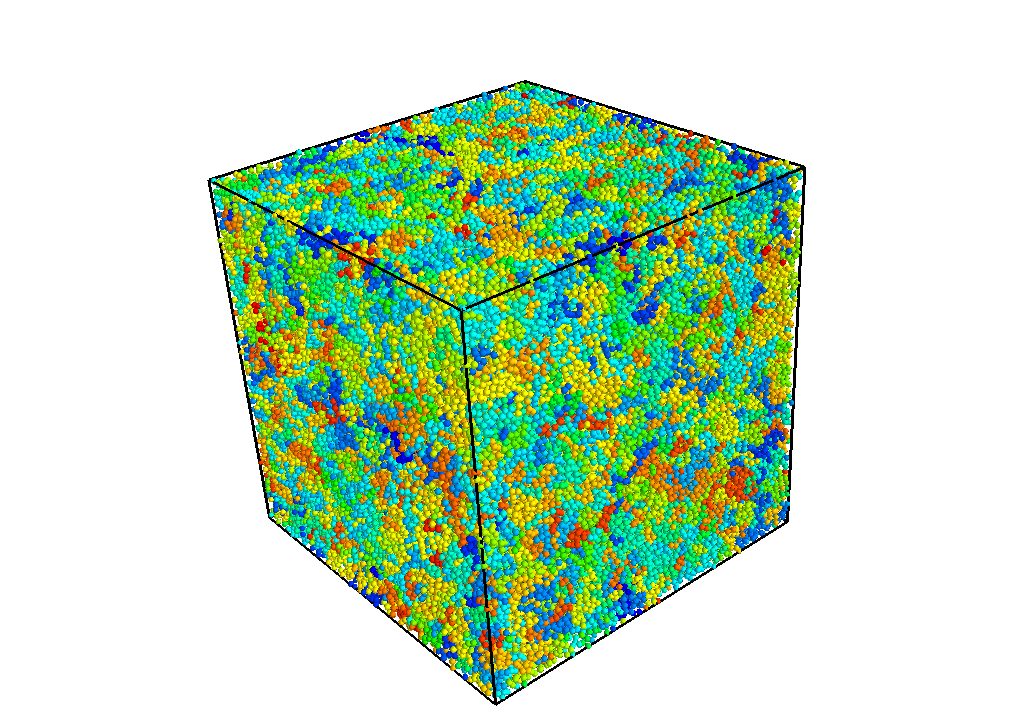
\includegraphics[keepaspectratio, width=1.01\paperwidth]{figs/fig-title_page_conf.png}
      };

      % BYU logo
      \node [draw=none, align=center, anchor=north west] 
        at ([xshift=-0.05in, yshift=0.05in] current page.north west)
      {
        
\includegraphics[keepaspectratio, width=0.75in]{./figs/BYU_IM22a.pdf}
      };

     % group logo
      \node [draw=none, align=center, anchor=north east] at (current page.north east)
      {
        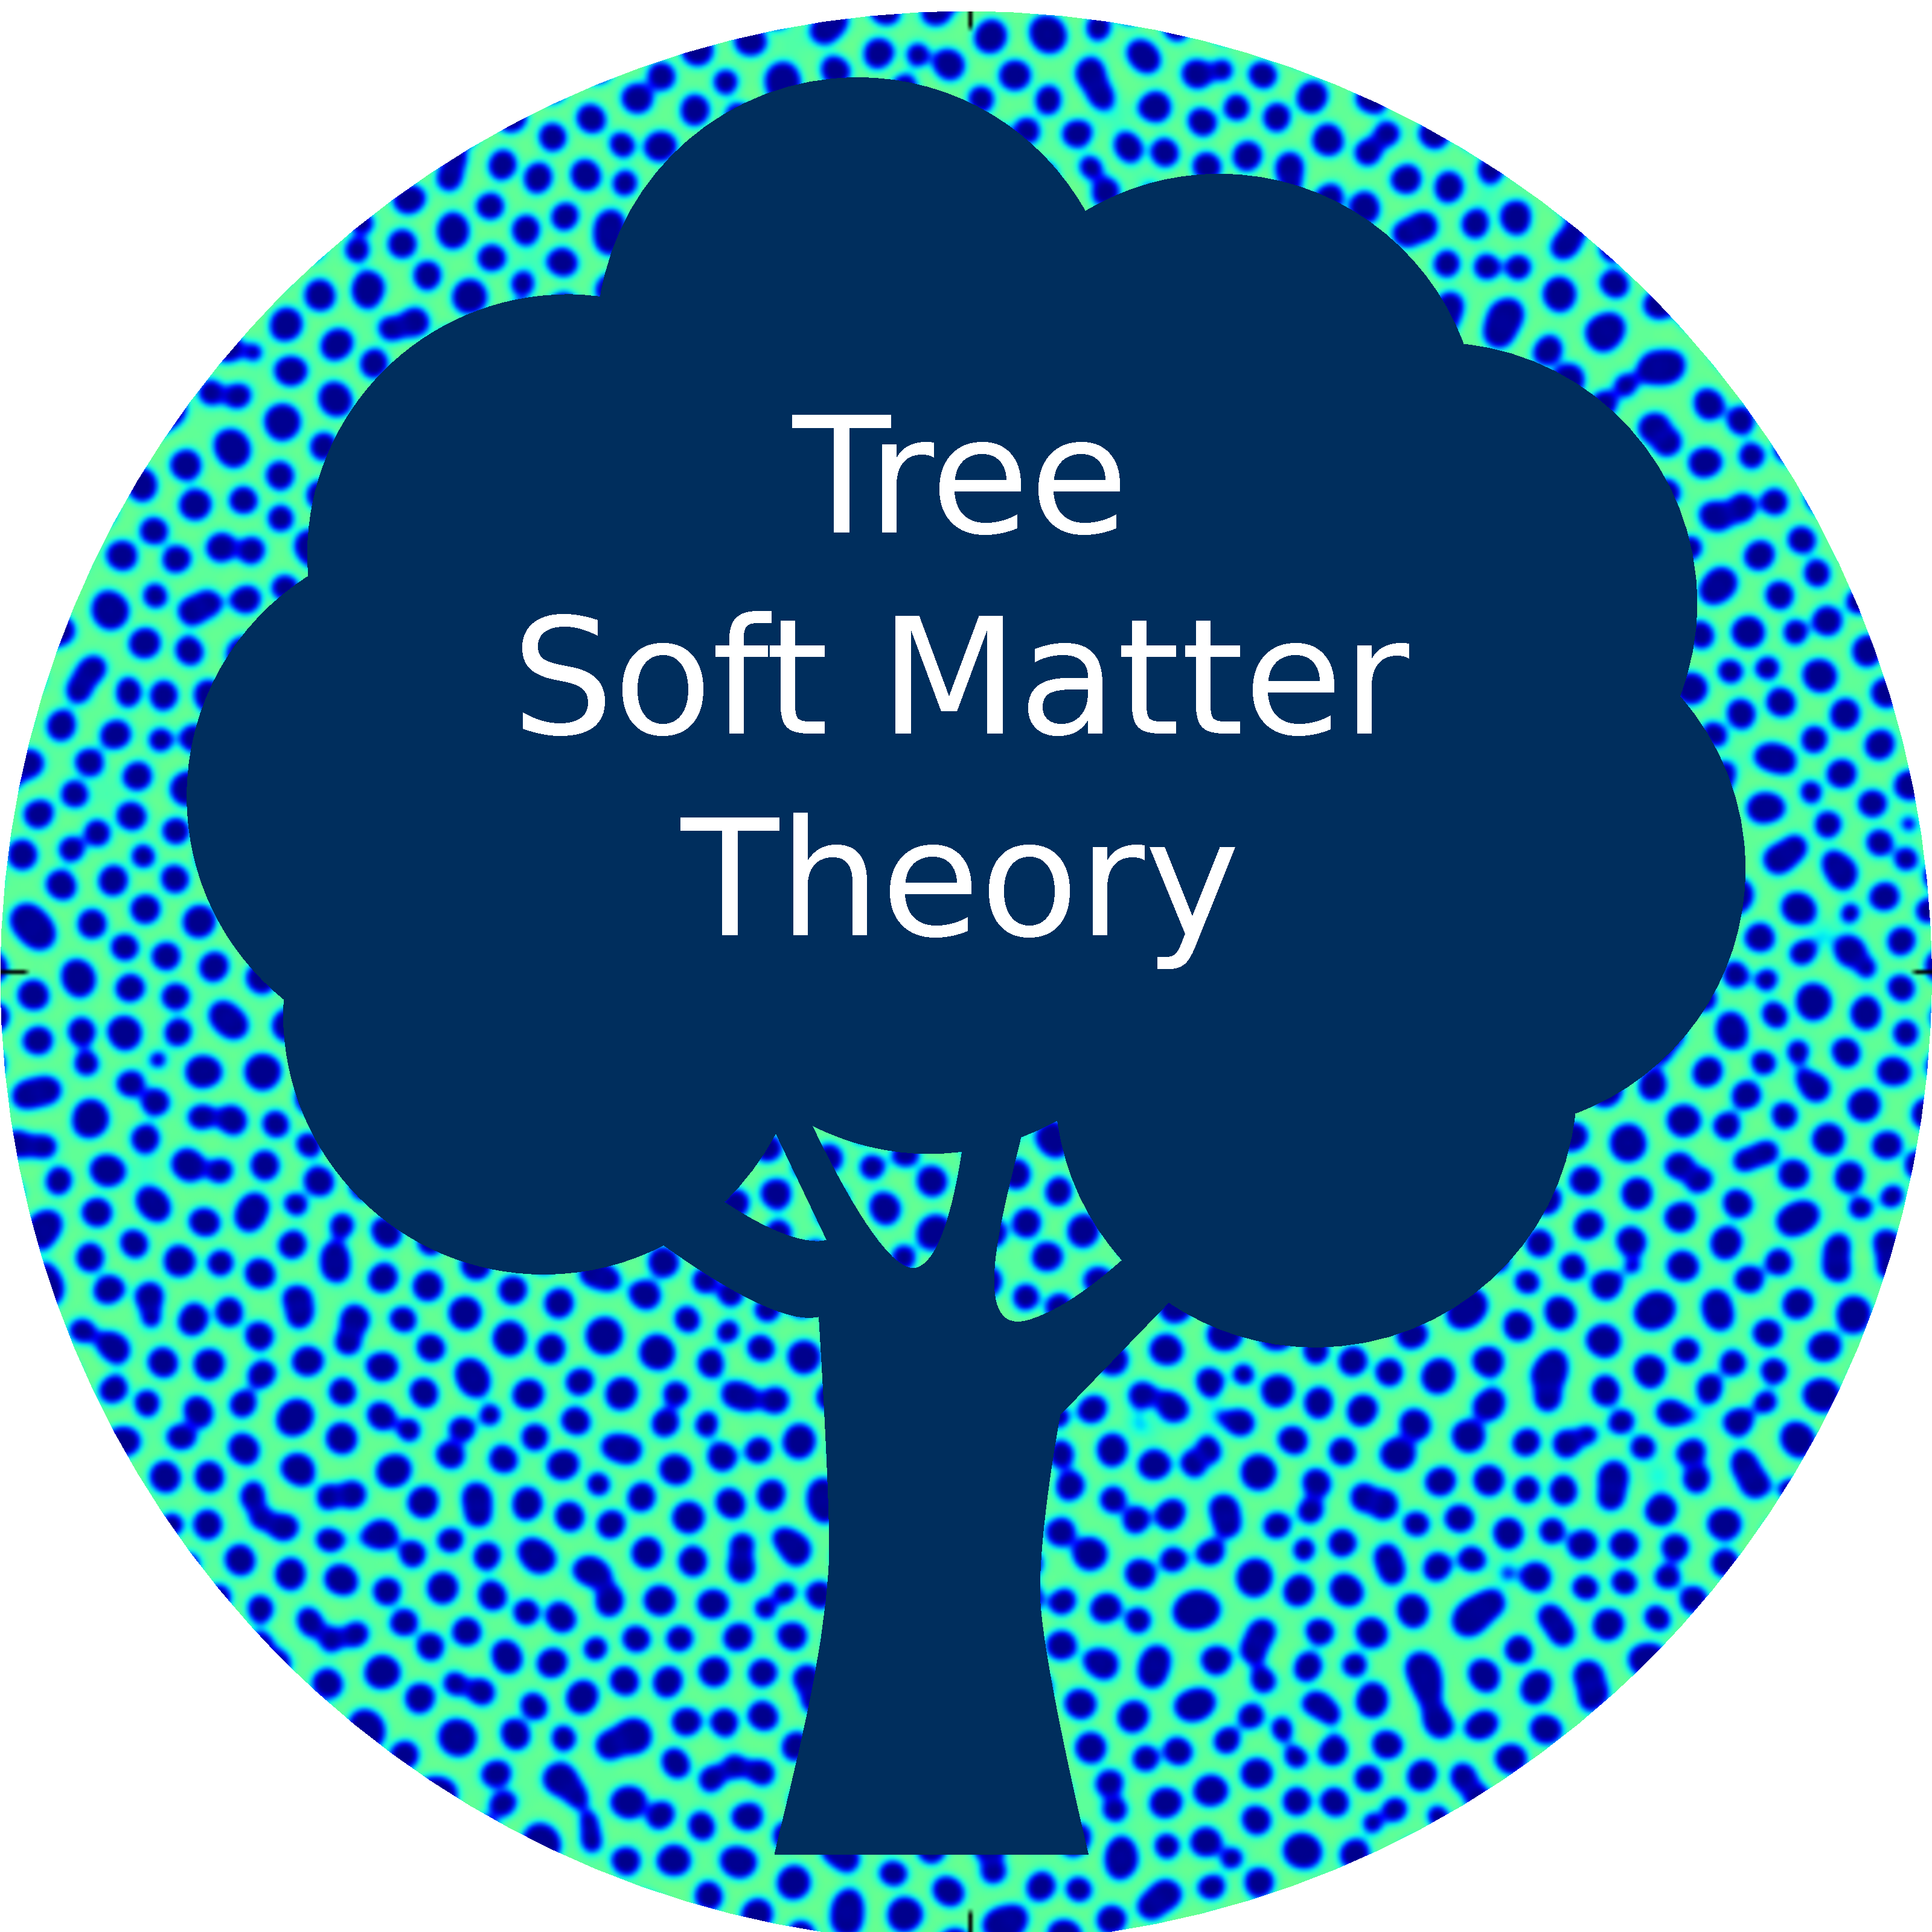
\includegraphics[keepaspectratio, width=0.6in]{./figs/TreeGroupLogo.pdf}
      };
  
      % title
      \usebeamercolor{title}
      \node [text width=0.85\paperwidth, align=center, draw=none, fill=black, rounded corners,
             fill opacity=0.6, text opacity=1, inner sep=5pt,
             below = 0.3in of current page.center, anchor=center] 
      {
        {
          \huge \titlecolor{} \inserttitle\par
        }
        \vspace{12pt}
        {
          \Large \bottomcolor{}\insertauthor \par
        } 
        \vspace{8pt}
        { 
          \bottomcolor{} \insertinstitute \par
        }

      };

      % add date
      \node [draw=none, text width=0.6\paperwidth, anchor=south west] (date)
      at (current page.south west)
      {
        \bottomcolor{}
        \raggedright
        \insertlocation\par
      };

      % add location
      \node [draw=none, above left = 0cm and 0cm of current page.south east, text width=0.6\paperwidth] (date)
      {
        \bottomcolor{}
        \raggedleft
        \insertdate\par
      };

    \end{tikzpicture}
    
}
% }}}

% ----- title/author info -----
\title{Simulation of Crystal \\Nucleation in Polymer Melts}
%\presenter{Pierre Kawak}
% for other authors
\author{Pierre Kawak}
\institute{Brigham Young University}
\location{\color{black}{Dissertation Defense}}
\date{\color{black}{June 29, 2022}}

\begin{document}

\begin{frame}[plain]
% Slide 0.1: Title
  % customize title page using the template in the preamble
  \titlepage
\end{frame}

\begin{frame}[t]{Let's address the elephant in the room}
%% {{{

  \centering
%  \begin{tikzpicture}
%    \node[text width=0.6\columnwidth, align=center, inner sep=0pt, xshift=-0.3] (A) {
%    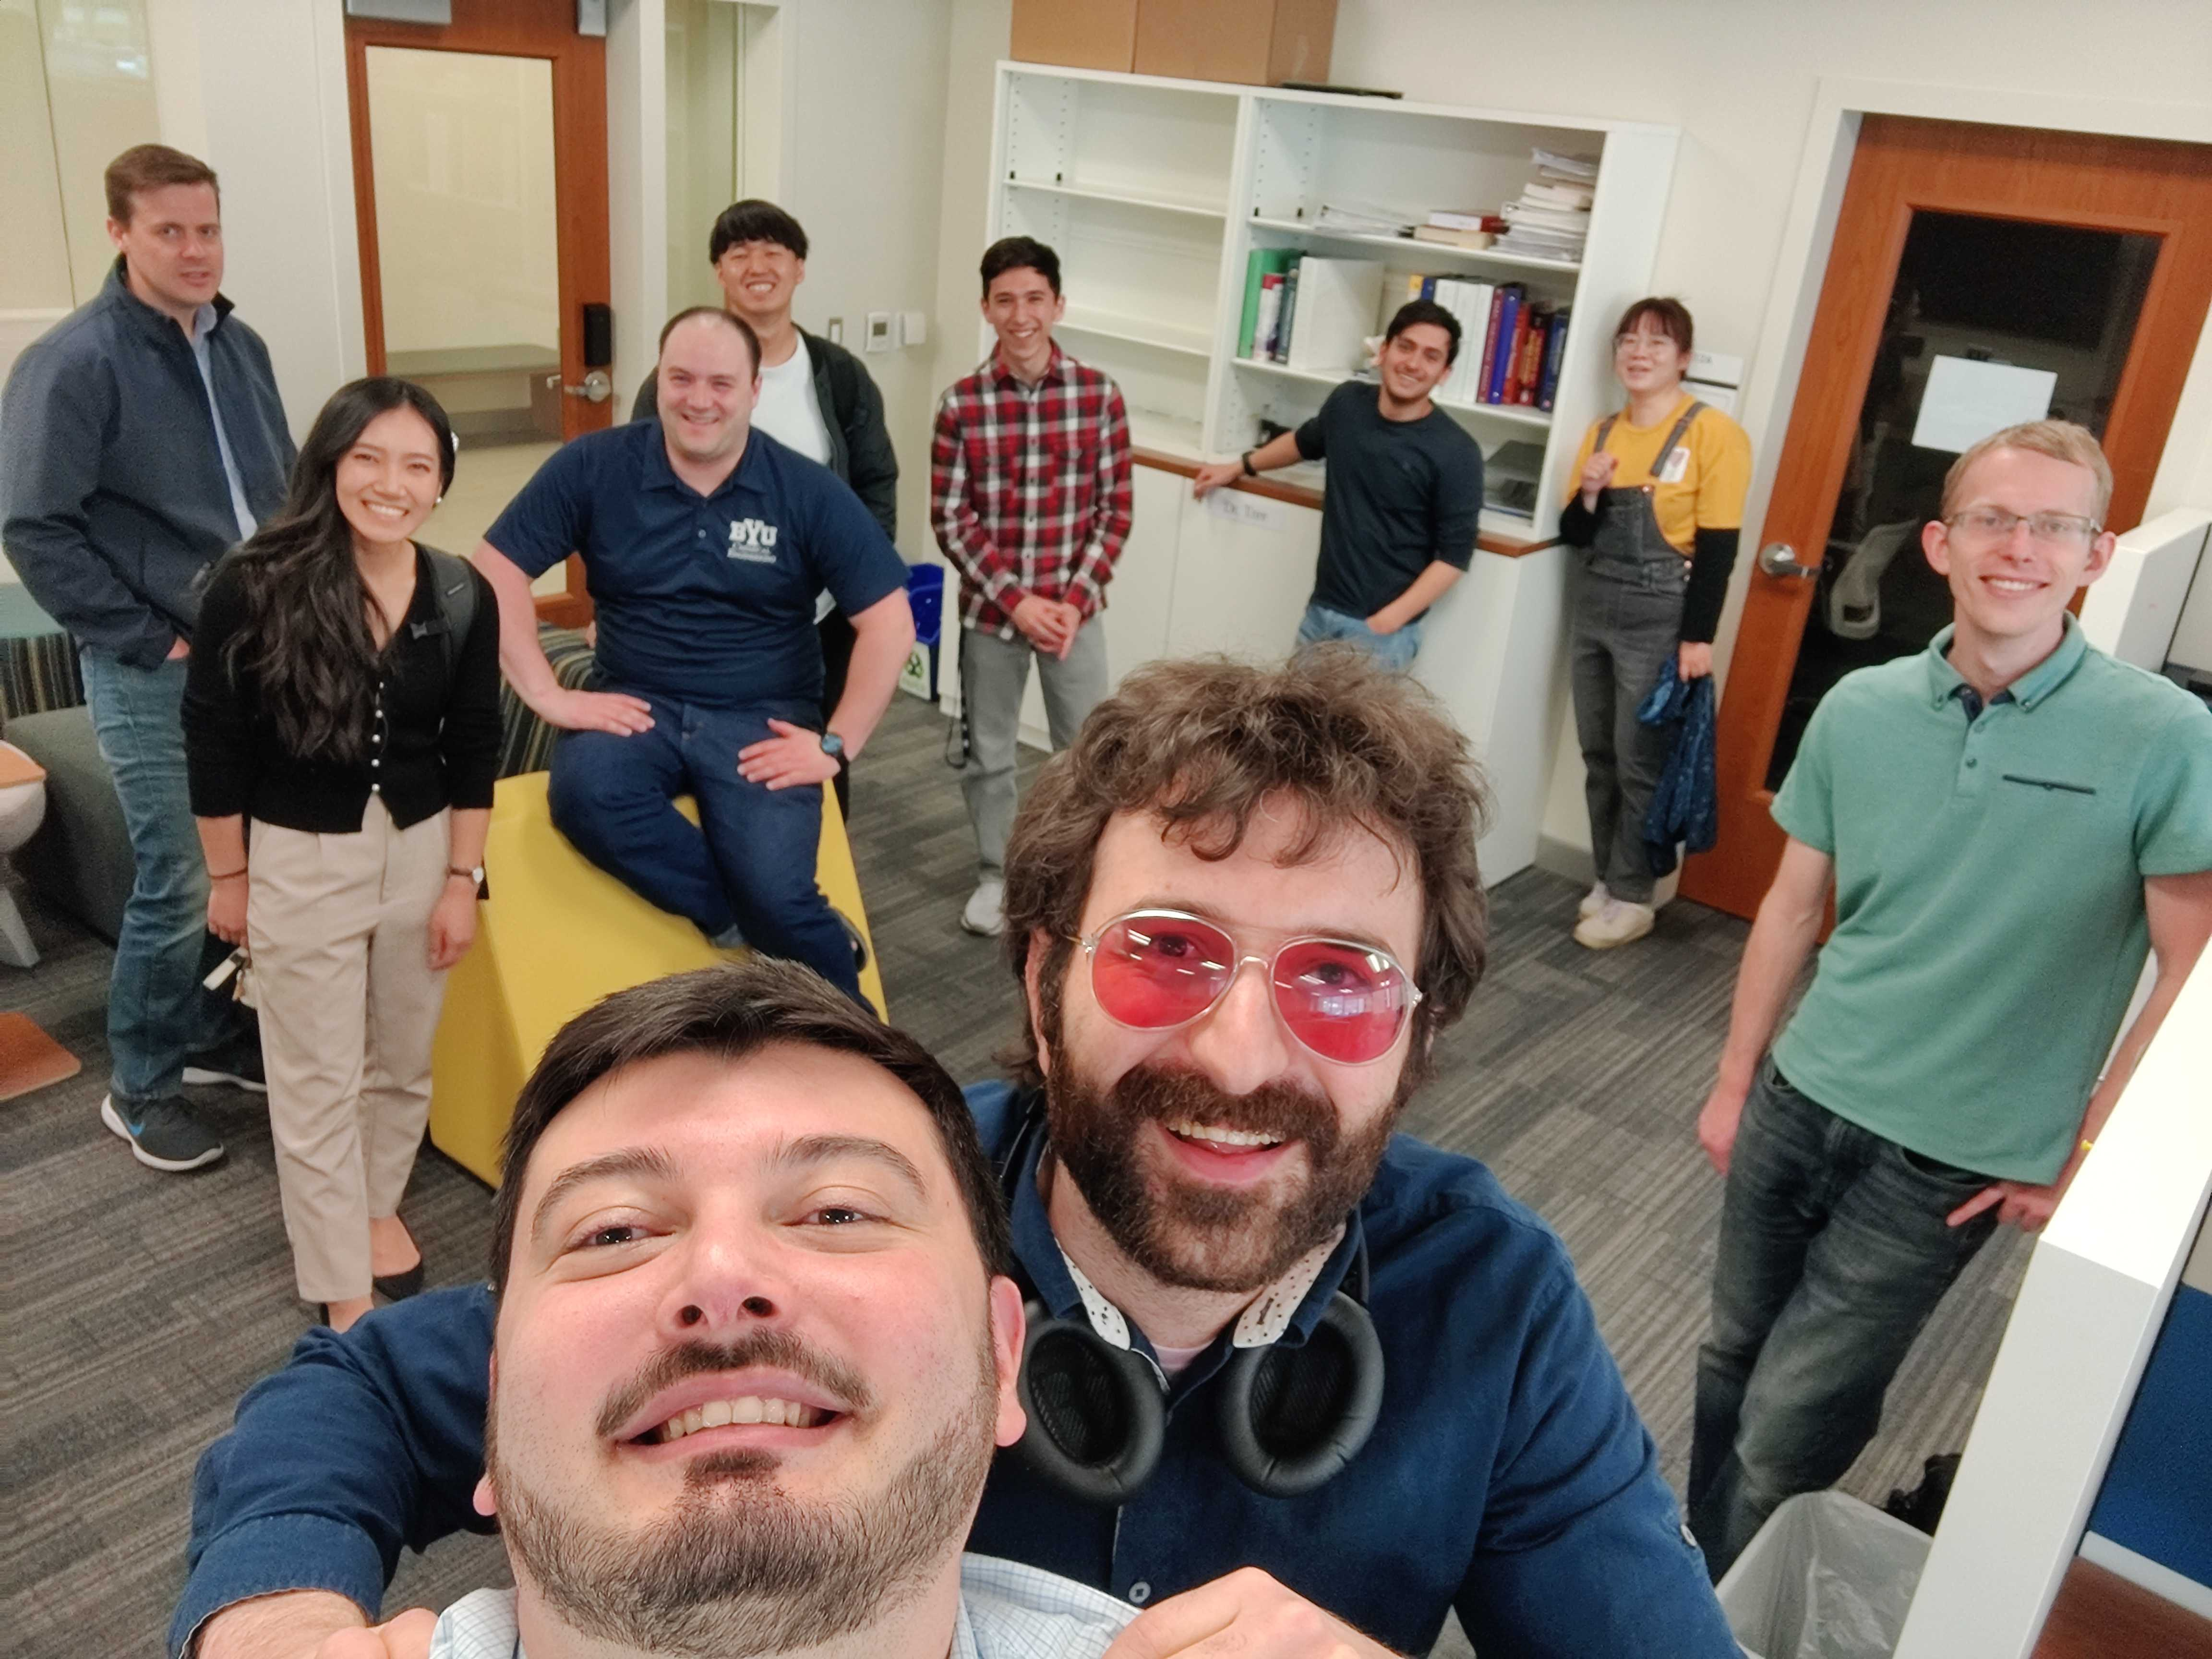
\includegraphics[width=\textwidth]{figs/Tree_Group_Photo_2022.jpg}
%    }; 
%
%    \node[text width=0.36\columnwidth, align=center, above left= 3.15cm and -6.0cm of A.east, anchor=north east, inner sep=0pt] (B) {
%    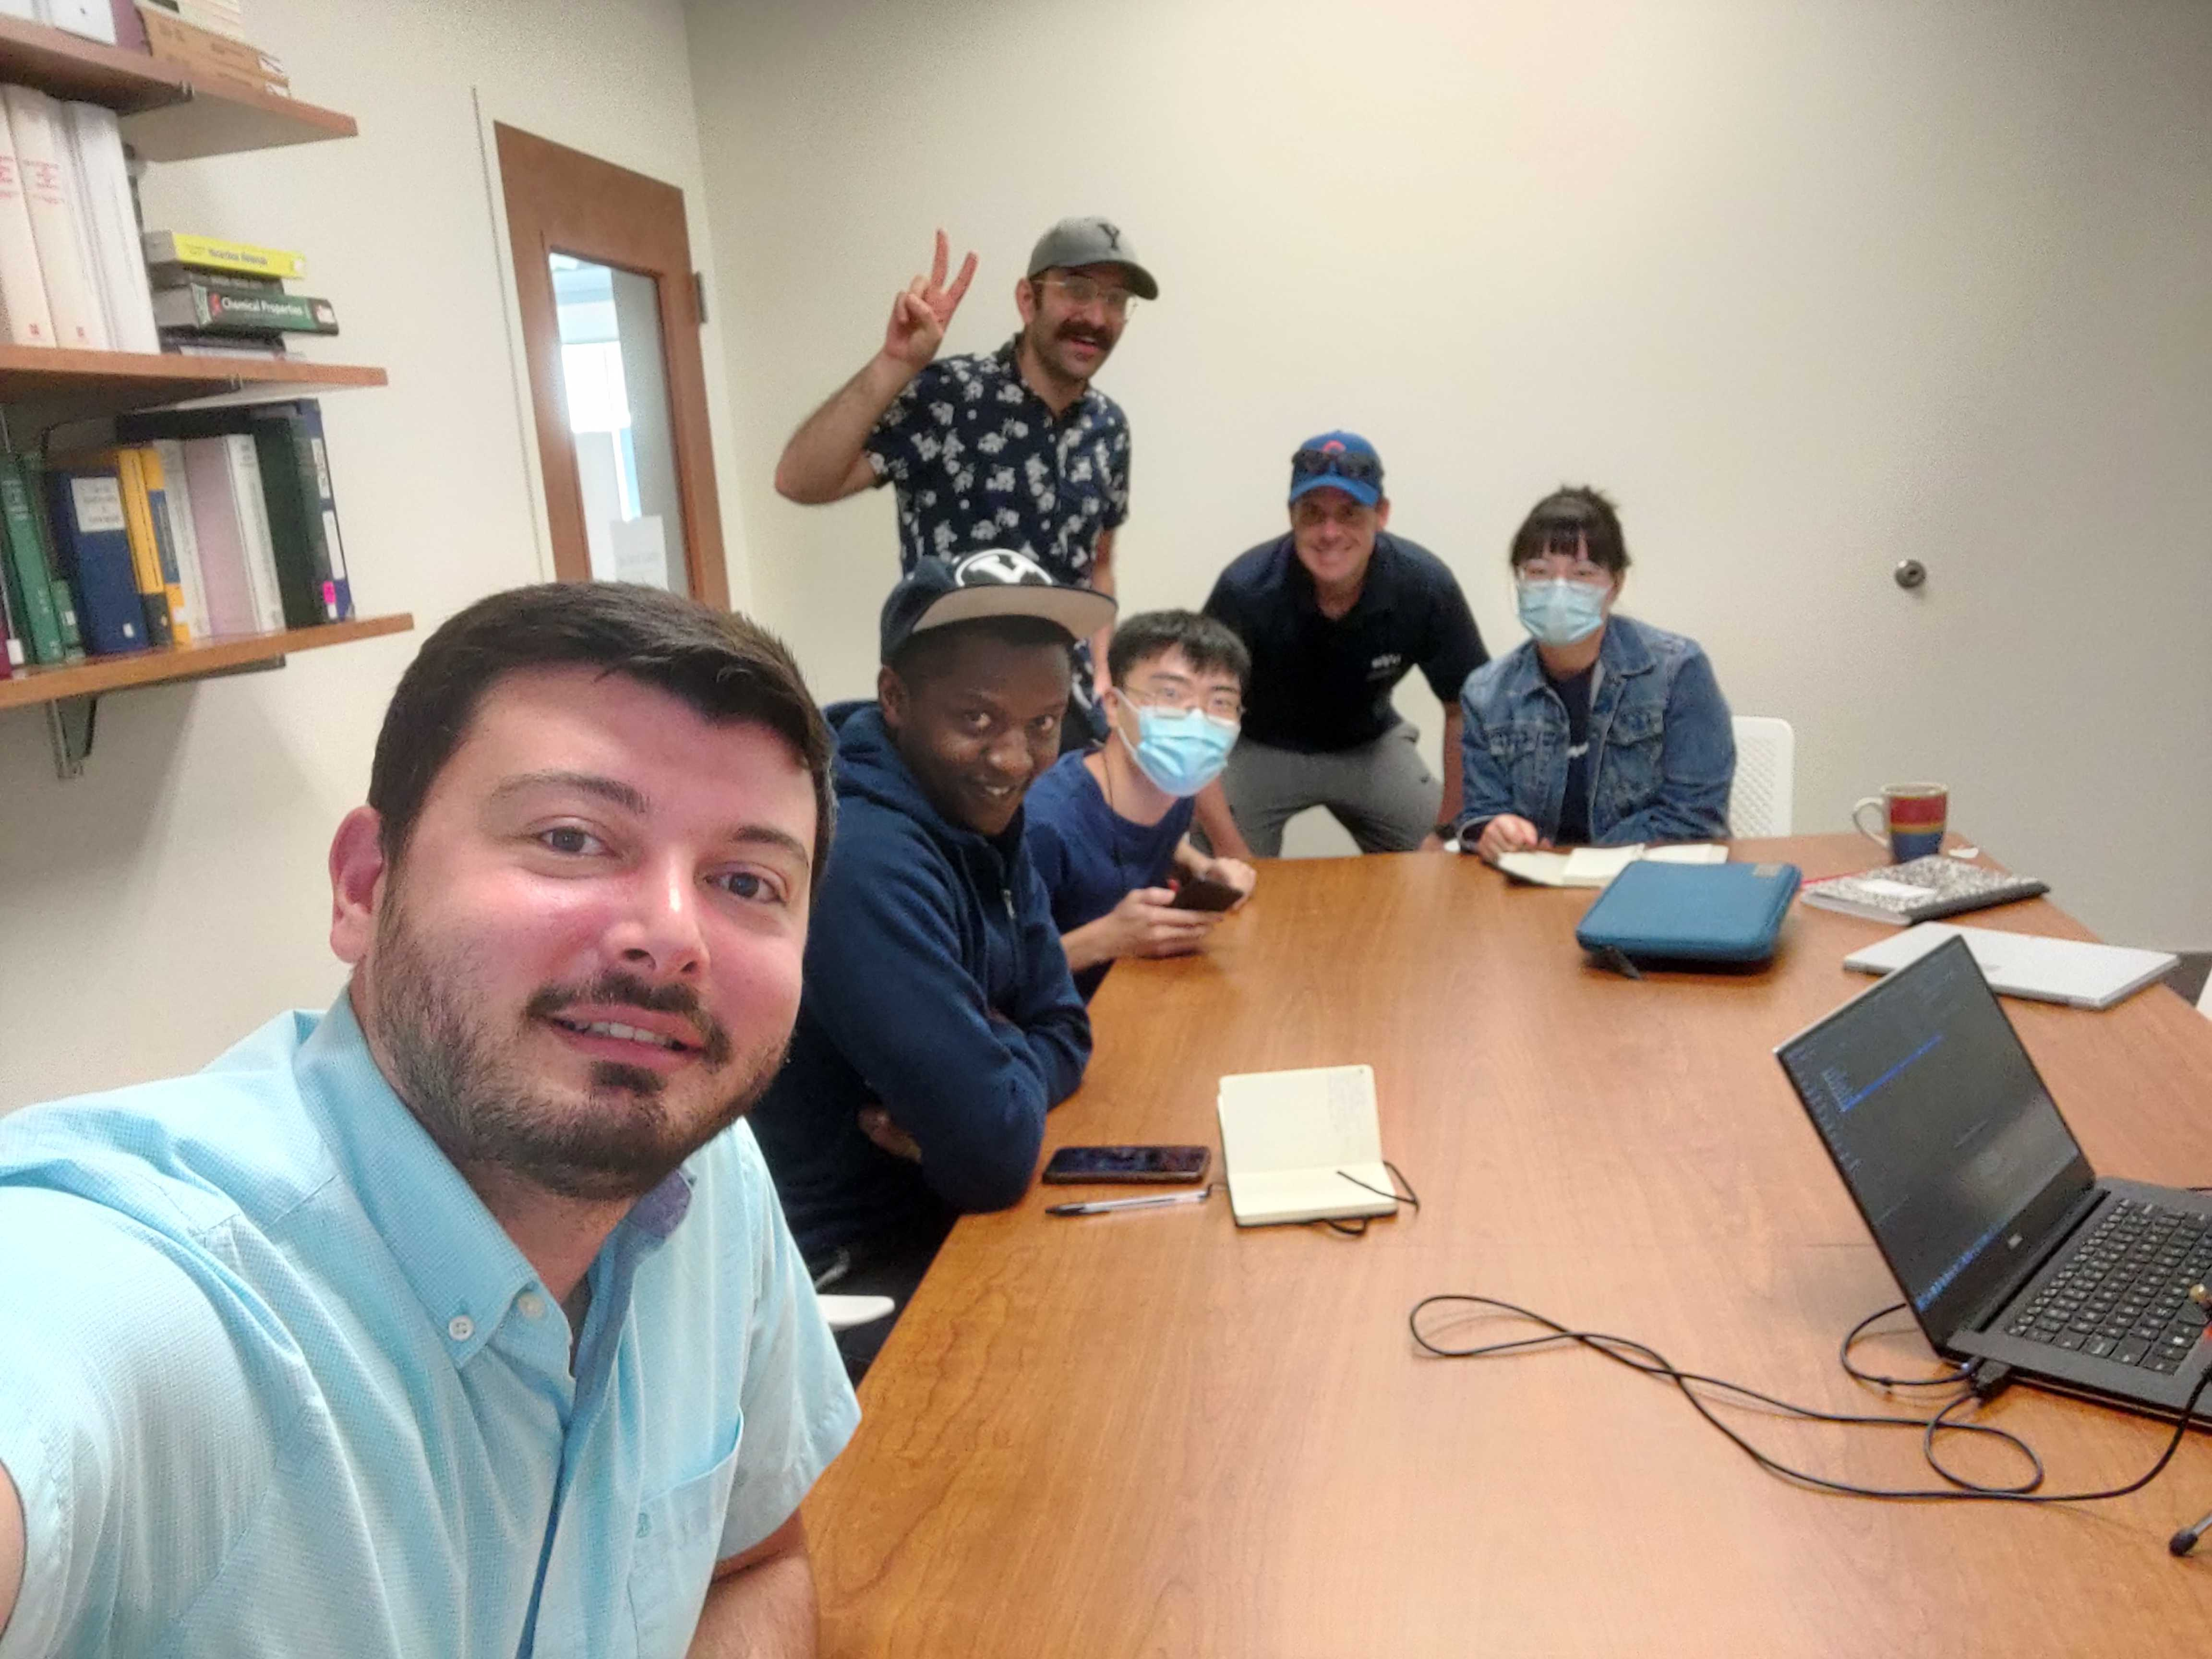
\includegraphics[width=\textwidth]{figs/GSC_Group_Photo_2021.jpg}
%    }; 
%
%    \node[text width=0.36\columnwidth, align=center, above left= -1.0cm and -6.0cm of A.east, anchor=north east, inner sep=0pt] (C) {
%    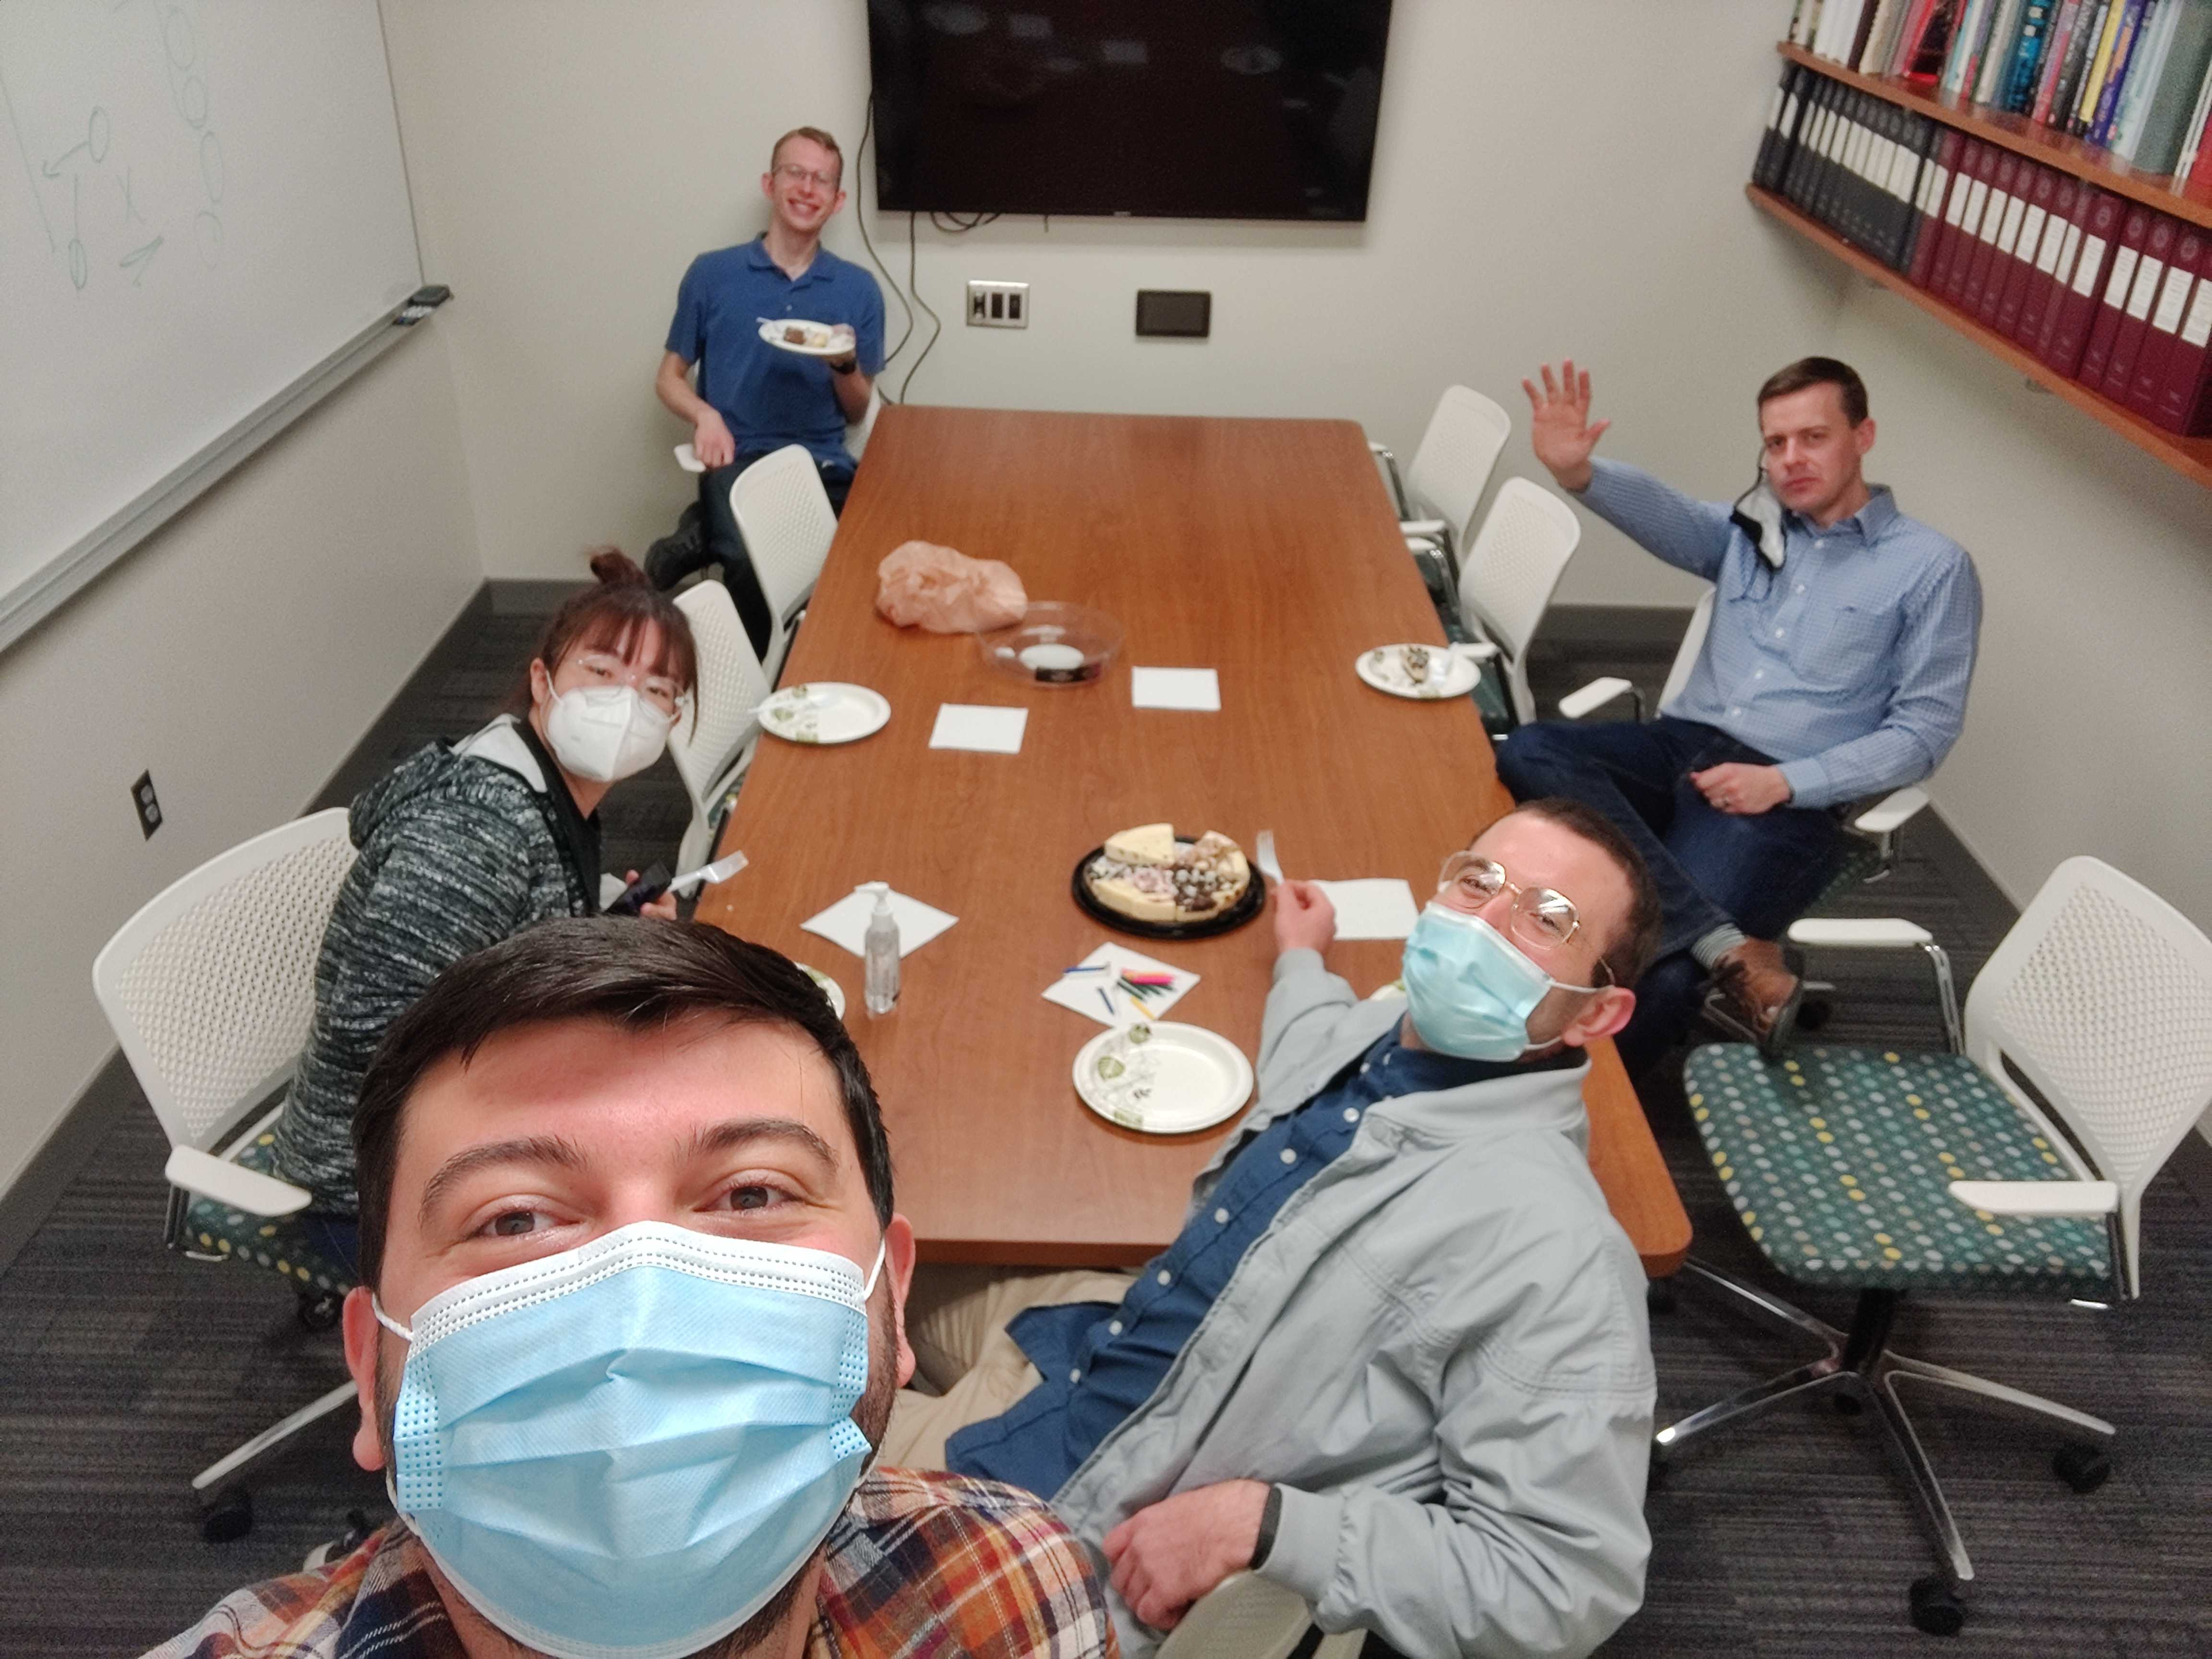
\includegraphics[width=\textwidth]{figs/Tree_Group_Photo_cake.jpg}
%    }; 
%
%  \end{tikzpicture}
  \only<2->{
  \begin{columns}[T]

  \column{0.39\textwidth}
    \centering

    \blocktitle{Samson}

    \vspace{\baselineskip}
    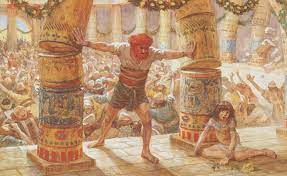
\includegraphics[trim=30 0 60 0, clip, height=5cm]{./figs/samson2.jpeg}

  \column{0.245\textwidth}
    \centering

    \blocktitle{Goku}

    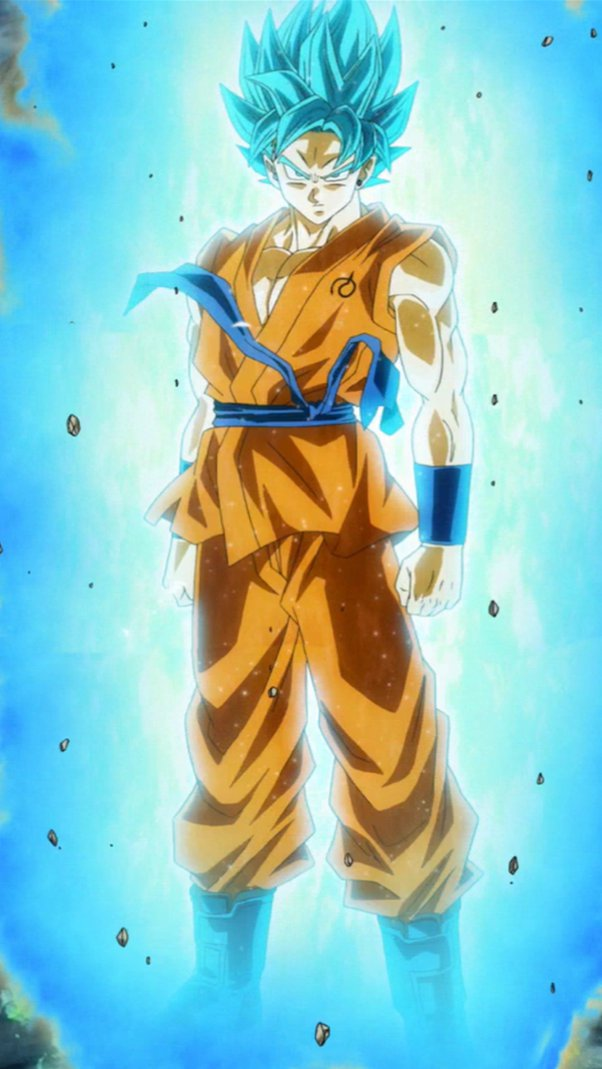
\includegraphics[height=5cm]{./figs/goku.jpeg}

  \column{0.245\textwidth}
    \centering

    \only<3>{
    \blocktitle{Me}

    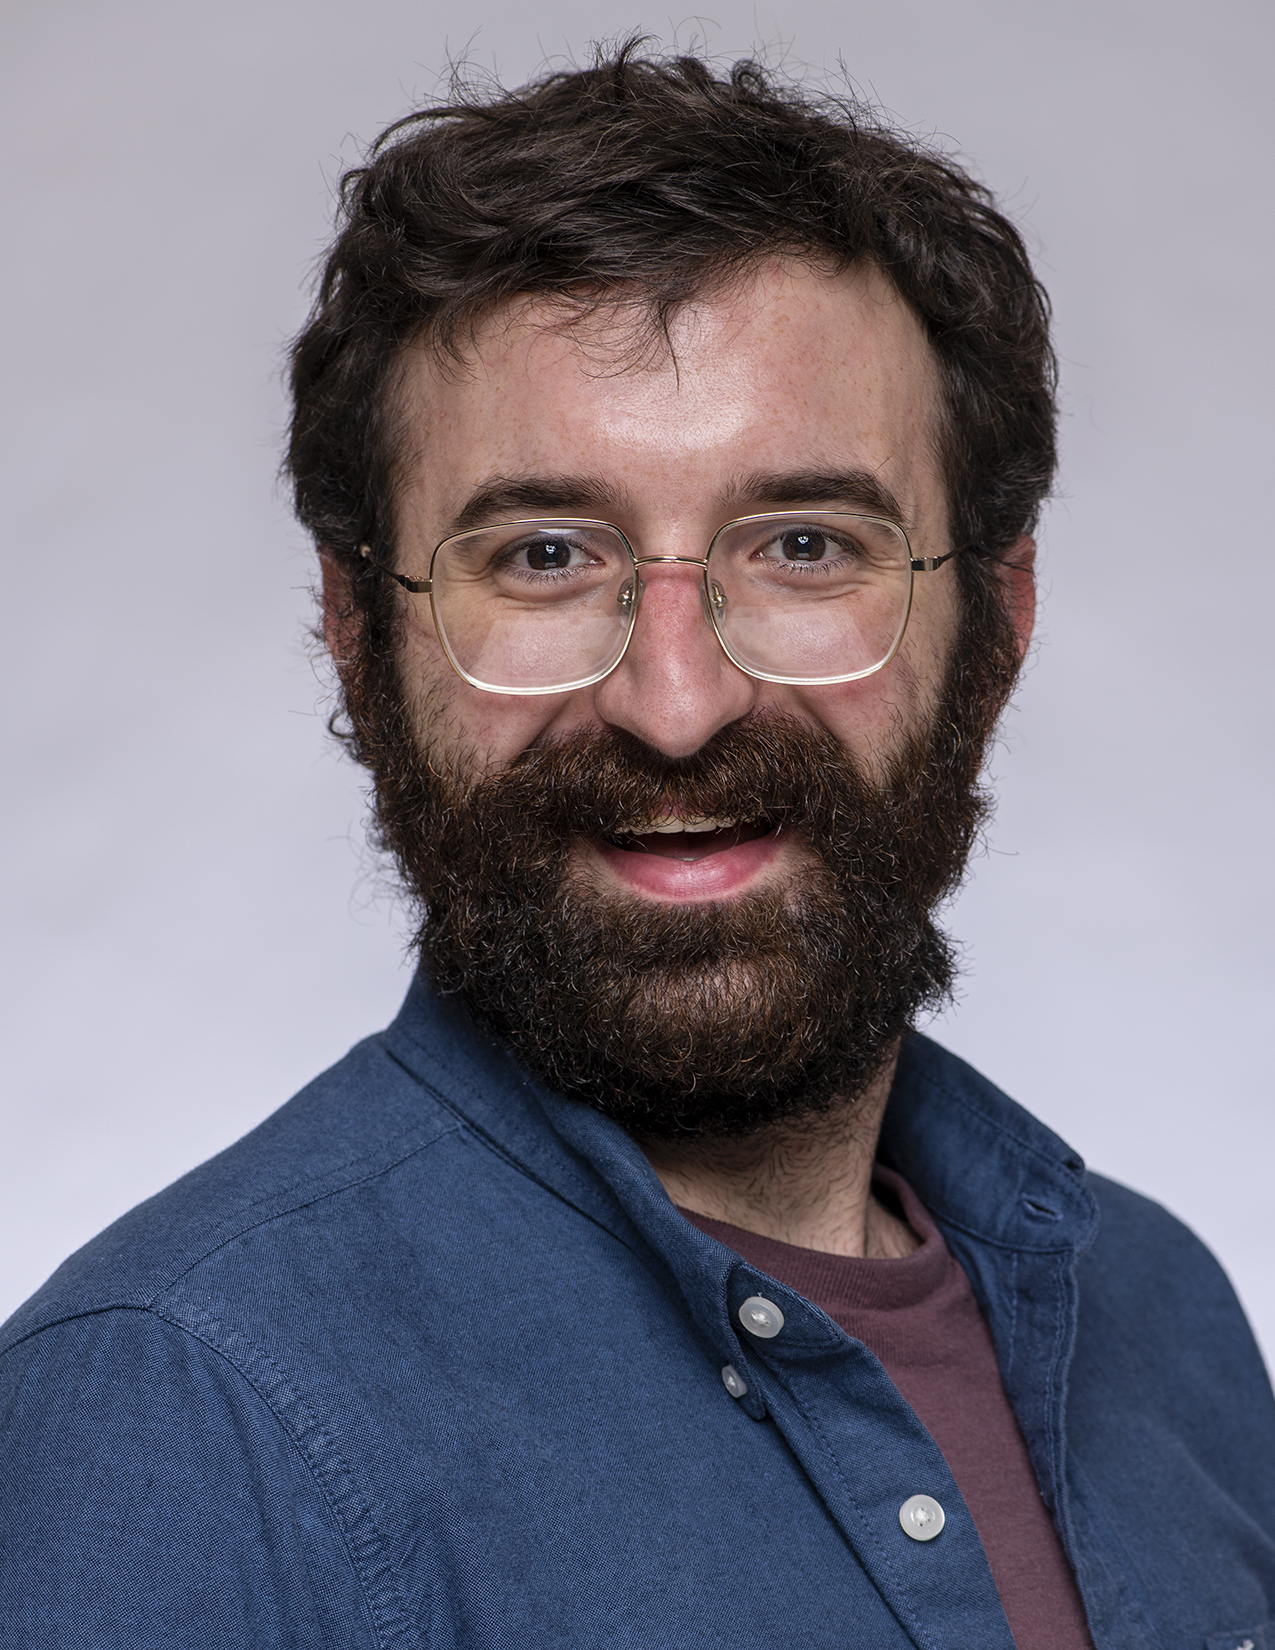
\includegraphics[height=5cm]{figs/Pierre_pic.jpg}
    }

  \end{columns}
  }

%% }}}
\end{frame}

% Section 0: Introduction
\begin{frame}[t]{Polymer properties depend on their crystallinity}
% Slide 0.2: The why? Polymers rule & cryst imp. to properties.
% {{{

  \vspace{1ex}
  \begin{columns}

    \column{0.5\textwidth}
      \centering
      \blocktitle{\% industrial production}
      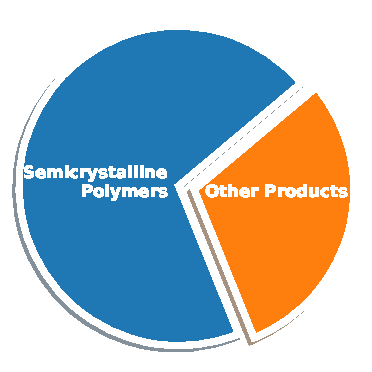
\includegraphics[]{figs/fig-semicrystal_fraction.pdf}

    \only<2>{
    \column{0.5\textwidth}
      \centering
      \blocktitle{Polyethylene product properties}
      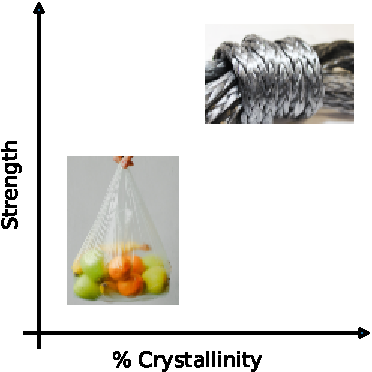
\includegraphics[]{figs/fig-cryst_props.pdf}
    }

  \end{columns}
% }}}
\end{frame}

\begin{frame}[t]{Molecular Dynamics (MD) suggests different crystal nucleation in polymers}
% {{{
% Slide 0.4 Varied results from NEMD sims.
  \vspace{-0.5\baselineskip}

  \begin{columns}[T]

  \column{0.5\textwidth}

    \centering
    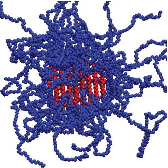
\includegraphics[height=0.5\textwidth]{figs/fig-Rutledge_crystal_crop.pdf}
    \vspace{0.5\baselineskip}

    \begin{block}{Non-equilibrium MD experiment 1}
      \begin{itemize}
        \item Cylindrical crystal nucleus
        \item Crystal size is a good order parameter
        \item No intermediate phases/states
        \item One-step crystallization
%        \item General agreement with classical models 
      \end{itemize}
    \end{block}

    \vspace{4pt}
    {\small{}Yi et al.~Macromolecules (2013)\par}

  \column{0.5\textwidth}

    \centering
    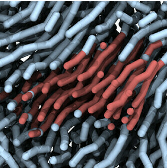
\includegraphics[height=0.5\textwidth]{figs/fig-Hall_crystal_crop.pdf}
    \vspace{0.5\baselineskip}

    \begin{block}{Non-equilibrium MD experiment 2}
      \begin{itemize}
        \item Crystal nucleus not cylindrical
        \item Crystal size is not only order parameter
        \item Crystal nucleates in nematic droplet
        \item Two-step crystallization
%        \item Disagrees with classical models
      \end{itemize}
    \end{block}

    \vspace{4pt}
    {\small{}Hall et al.~J.~Phys.~Chem.~B.~(2020)\par}

  \end{columns}

  \onslide<2>{
  \begin{tikzpicture}[remember picture, overlay]

    \node[fill=white, minimum width=10cm, minimum height=3cm, 
          rounded corners=0.2cm, anchor=center, opacity=0.7] 
          at (current page.center) {
    };

    \node[text width=9cm, fill=lightblue, draw=darkblue, very thick, rounded corners=0.2cm, anchor=center] 
          at (current page.center) {
    The controversy extends to:
    \begin{itemize} 
      \item Dynamic SAXS/WAXS measurements
      \item Recrystallization and melt memory experiments
      \item Direct observations of precursors
    \end{itemize}
    };

  \end{tikzpicture}
  }

% }}}
\end{frame}

\begin{frame}[c]{Contradictions in simulations (and experiments) have led to new theories}
% {{{
% Slide 0.5: Contradictions in simulations (and experiments) have led to new theories

  \begin{columns}[T]

  \column{0.5\textwidth}

    \centering
    \blocktitle{Classical Nucleation Theory for Polymers}

    \vspace{0.2\baselineskip}
    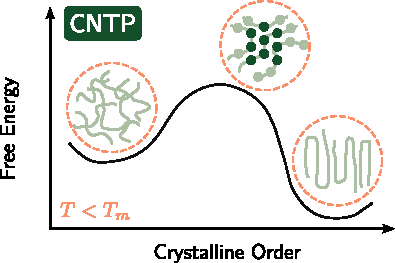
\includegraphics[scale=1.05]{figs/fig-CNTP_Free_Energy.pdf}

    \vspace{0.65\baselineskip}
    {\scriptsize 
    Lauritzen and Hoffman.~J.~Chem.~Phys.~(1959)\par
    Lauritzen and Hoffman.~J.~Appl.~Phys.~(1973)\par
    Schultz.~Polym. Cryst.~(2001)\par
    Yi et al.~J.~Chem.~Phys.~(2009)\par
    }

  \column{0.5\textwidth}

    \centering
    \blocktitle{``SOMM'' Hypothesis}
    \vspace{1.2\baselineskip}

    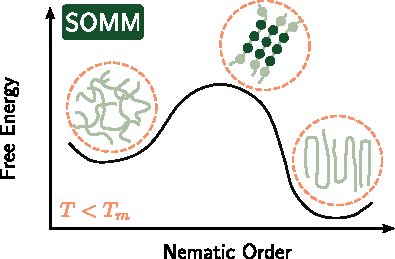
\includegraphics[scale=1.05]{figs/fig-SOMM_Free_Energy.pdf}

    \vspace{0.7\baselineskip}
    {\scriptsize 
    Strobl.~The Physics of Polymers.~(2007)\par
    Olmsted.~Phys.~Rev.~Lett.~(1998)\par
    Milner.~Soft Matter.~(2011)\par
    Welch and Muthukumar.~Phys.~Rev.~Lett.~(2001)\par
    }
  
  \end{columns}
%TODO add references

% }}}
\end{frame}

\begin{frame}[c]{A way forward? Calculate the free energy landscape (FEL) at equilibrium}
% {{{
% Slide 0.6: A way forward? Calculate the free energy landscape (FEL) at equilibrium

  % Key idea
  \begin{columns}[T, onlytextwidth]
  
  \column{0.50\textwidth}

    \centering

    \vspace{-0.5\baselineskip}
    \begin{block}{Key idea}
      \begin{itemize}
        \item All theories are based on a \emph{free energy landscape}
        \item An FEL is a \emph{near-equilibrium} concept
      \end{itemize}
    \end{block}

  \column{0.47\textwidth}
    \centering
    \vspace{-12pt}
    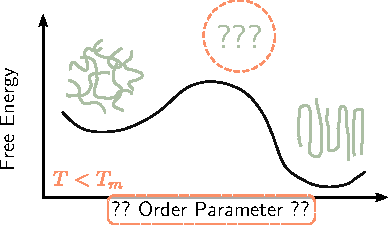
\includegraphics[width=0.8\textwidth]{figs/fig-key_idea_shorter.pdf}
  
  \end{columns}

  \vspace{15pt}

  % Our approach
  \begin{columns}[T, onlytextwidth]
  
  \column{0.50\textwidth}

    \centering

    \vspace{-0.5\baselineskip}
    \begin{block}{Our Approach}
      Use \emph{equilibrium Monte Carlo} methods
      \begin{itemize}
        \item Avoid kinetic traps in MD
        \item Identify (meta)stable phases
        \only<1>{\item Study crystalline and nematic order}
        \only<2>{\item Study crystalline and nematic order}
        \item Calculate free energy landscapes
      \end{itemize}
    \end{block}

%    \onslide<3>{
%      \begin{tikzpicture}[remember picture, overlay]
%        \node[minimum width=7cm, minimum height=1.75cm, fill=white, opacity=0.7] 
%             at ([xshift=-4.0cm, yshift=-0.88cm] current page.center) {
%        };
%      \end{tikzpicture}
%    }

  \column{0.47\textwidth}
    \centering
   % 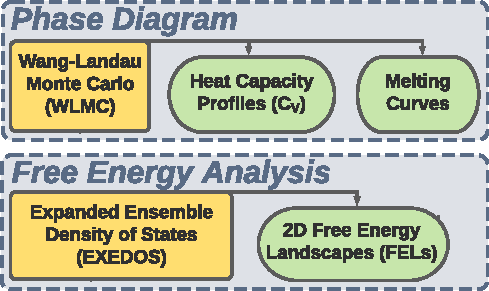
\includegraphics[width=0.9\textwidth]{figs/fig-MCFEL_simple.pdf}
    \vspace{3.5\baselineskip}
    \vspace{5pt}

    \begin{tikzpicture}[remember picture, overlay]

      \node[] { 
        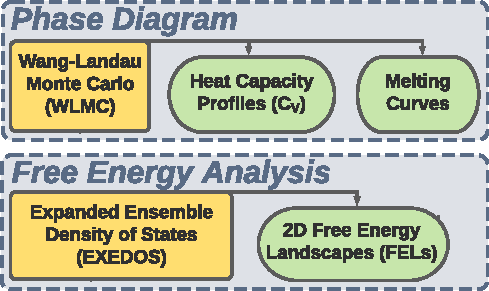
\includegraphics[width=0.9\textwidth]{figs/fig-MCFEL_simple.pdf}
      };

    \end{tikzpicture}
    \only<1>{
      \begin{tikzpicture}[remember picture, overlay]
          \node[minimum width=14cm, minimum height=4.0cm, fill=white, opacity=1.0] 
               at ([xshift=-0.3cm, yshift=-1.8cm] current page.center) {
          };

      \end{tikzpicture}
    }
  
  \end{columns}

%  \par
%
%  \begin{tikzpicture}[remember picture, overlay]
%    \node[text width=8cm, align=center, anchor=south] at ([yshift=0.1cm] current page.south) {
%      \scriptsize{}Kawak, Banks, \& Tree.~J.~Chem.~Phys. (2021)\par
%    };
%  \end{tikzpicture}

% }}}
\end{frame}

%%\begin{frame}[c]{Melt memory is indicative of unusual crystallization behavior in polymer melts}
%%% {{{
%%% Slide 1: Use Hafele example + other observations slide
%%
%%  \begin{columns}[T]
%%
%%  \column{0.64\textwidth}
%%
%%    \centering
%%%how do I move it to the left
%%    \onslide<1->{
%%    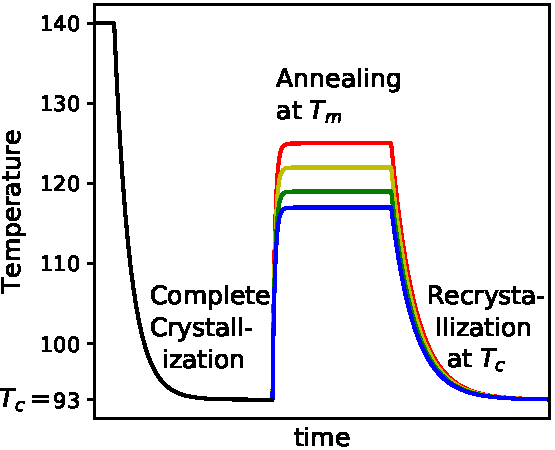
\includegraphics[]{figs/fig-melt_mem.pdf}
%%    }
%%
%%  \column{0.36\textwidth}
%%
%%    \centering
%% %   \hspace{-30pt}
%%    \only<2>{
%%    \vspace{2.0\baselineskip}
%%    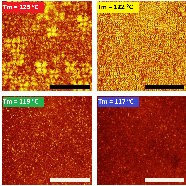
\includegraphics[width=1.1\textwidth]{figs/colored_melt_mem.pdf}
%%    }
%%    
%%    \onslide<3>{
%%    \vspace{1.0\baselineskip}
%%    \begin{block}{Other Observations}
%%      \begin{itemize} 
%%        \item Initial larger scale ordering in SAXS/WAXS measurements
%%        \item Deviant Crystallization and Recrystallization line
%%        \item Intermediate Phase Observations
%%        \item No Copolymer Effect on Crystallization
%%      \end{itemize}
%%    \end{block}
%%    }
%%
%%  \end{columns}
%%%% }}}
%%\end{frame}

%\begin{frame}[t]{The problem: Simulations at equilibrium are difficult and take long times}
%% {{{
%% Slide 0.5 Our approach: - Equilibrium MC sims of polymer crystal CG models.
%\centering
%% }}}
%\end{frame}
%

\begin{frame}<1-2>[t, label=outline]{Outline}
% {{{
% Slide 0.7: The outline

  \tikzstyle{boxstyle} = [
          draw=darkblue,
          fill=none,
          thick,
          rounded corners,
          minimum width=3.65cm,
          minimum height=3.41cm,
          text width=6.25cm,
          align=center,
          text=black
          ]

  \tikzstyle{dblbox} = [
          draw=darkblue,
          fill=none,
          thick,
          rounded corners,
          minimum width=3.65cm,
          minimum height=7.35cm,
          text width=6.25cm,
          align=center,
          text=black
          ]

  \tikzstyle{hilite} = [
          draw=darkblue,
          fill=lightorange,
          fill opacity=0.15,
          text opacity=1,
          thick,
          rounded corners,
          minimum width=3.5cm,
          minimum height=3.41cm,
          text width=6.25cm,
          align=center,
          text=black
          ]

  \vspace{6pt}
  \begin{tikzpicture}

    \node[text width=6.25cm] (anchor) {};

    \node[boxstyle, below right=0cm and 0cm of anchor.north west, anchor=north west] (crystallization)
    {
      Molecular Simulation Methods\\[5pt]
      \begin{minipage}{.4\textwidth}
      %  \centering
        \raggedright

        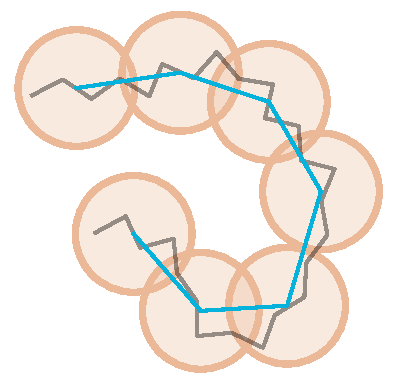
\includegraphics[width=\textwidth, angle=90, origin=c]{figs/subfig-long_CG_PE.pdf}
      \end{minipage}
      \begin{minipage}{.4\textwidth}
        \raggedleft

        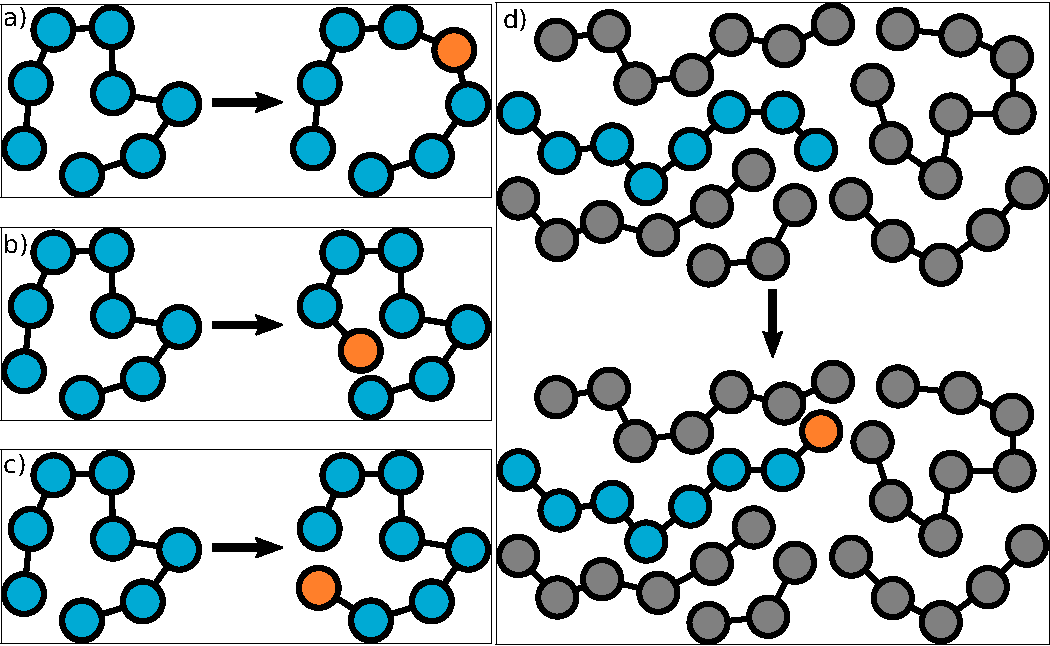
\includegraphics[trim=0 100 267 0, clip, width=\textwidth]{../figures/ch2_method/fig-polymer_moves/fig-polymer_moves.pdf}
      \end{minipage}
    };

    \only<2>{
    \node[hilite, below right=0cm and 0cm of anchor.north west, anchor=north west] (crystallization)
    {
      Molecular Simulation Methods\\[5pt]
      \begin{minipage}{.4\textwidth}
      %  \centering
        \raggedright

        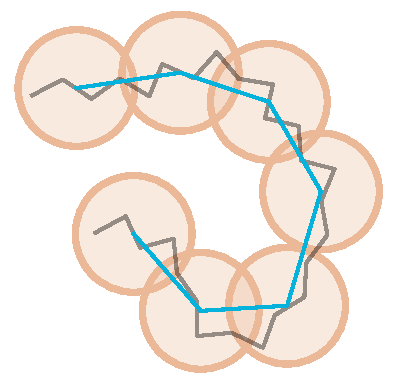
\includegraphics[width=\textwidth, angle=90, origin=c]{figs/subfig-long_CG_PE.pdf}
      \end{minipage}
      \begin{minipage}{.4\textwidth}
        \raggedleft

        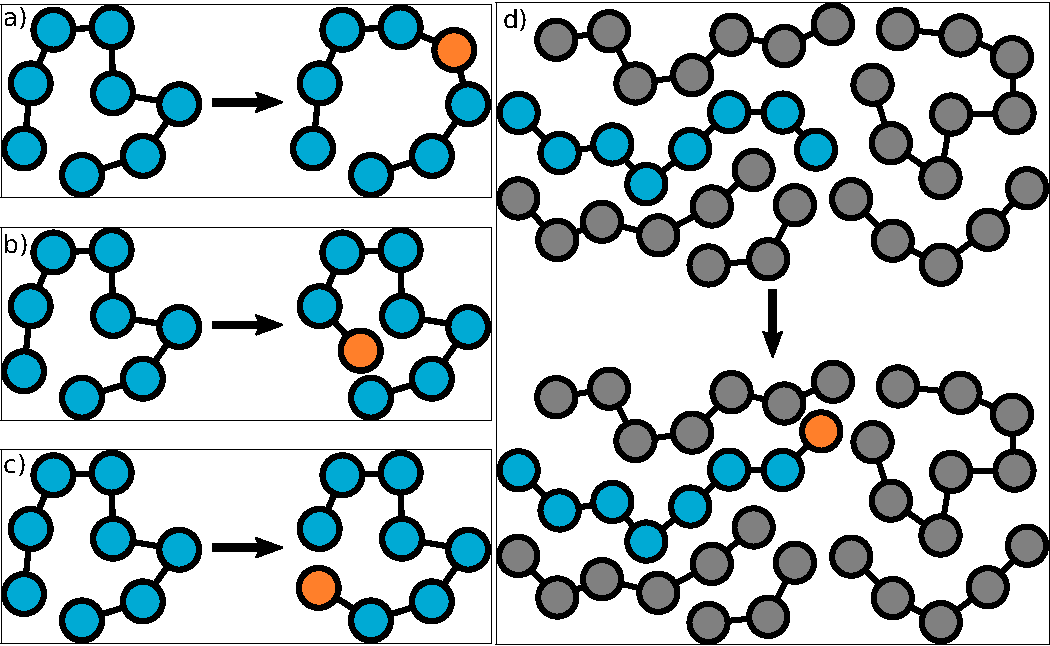
\includegraphics[trim=0 100 267 0, clip, width=\textwidth]{../figures/ch2_method/fig-polymer_moves/fig-polymer_moves.pdf}
      \end{minipage}
    };
    }

    \node[boxstyle, below=0.5 of crystallization] (y3)
    {
      Nucleation in a semiflexible oligomer\par
      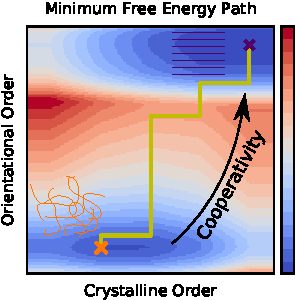
\includegraphics[width=0.45\textwidth]{figs/fig-pathway_ToC_chains.pdf}
    };

    \only<4>{
    \node[hilite, below=0.5 of crystallization] (y3)
    {
      Nucleation in a semiflexible oligomer\par
      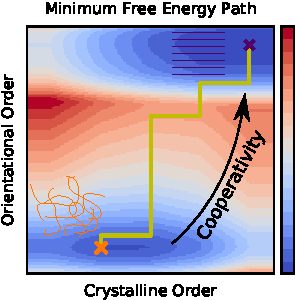
\includegraphics[width=0.45\textwidth]{figs/fig-pathway_ToC_chains.pdf}
    };
    }

    \node[boxstyle, right=0.5cm of anchor.north east, anchor=north west] (vesicles)
    {
      GPU-accelerated Monte Carlo\par
%      \vspace{\baselineskip}
      \begin{minipage}{.4\textwidth}
      %  \centering
        \raggedright
        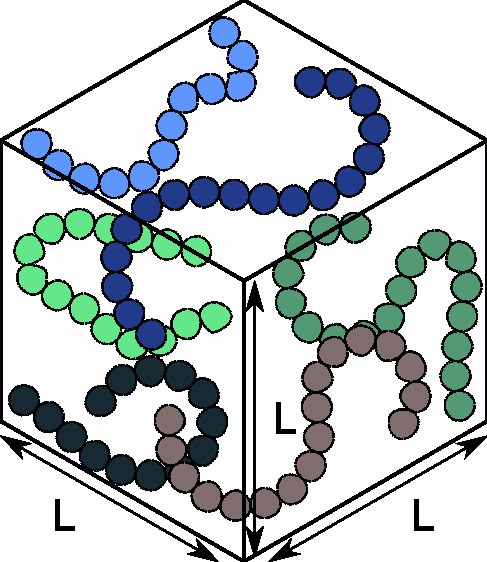
\includegraphics[width=0.95\textwidth]{figs/just_cube_wdims_wpols.pdf}
      \end{minipage}
      \begin{minipage}{.4\textwidth}
        \raggedleft
        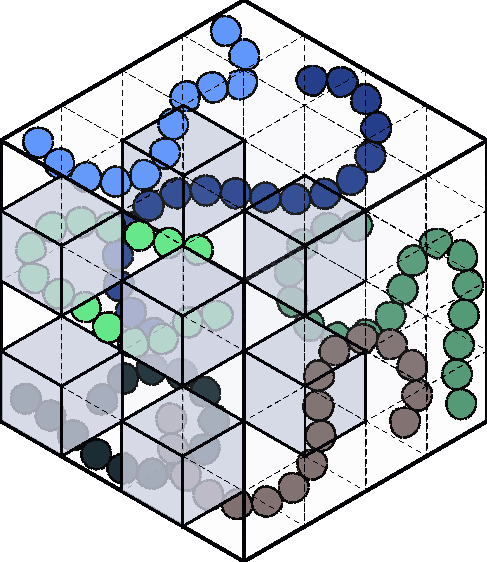
\includegraphics[width=0.95\textwidth]{figs/checkerboard_cube_wpols.pdf}
      \end{minipage}
    };

    \only<3>{
    \node[hilite, right=0.5cm of anchor.north east, anchor=north west] (vesicles)
    {
      GPU-accelerated Monte Carlo\par
%      \vspace{\baselineskip}
      \begin{minipage}{.4\textwidth}
      %  \centering
        \raggedright
        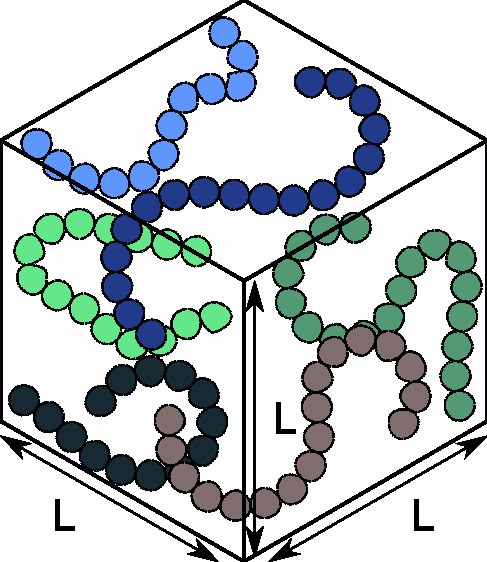
\includegraphics[width=0.95\textwidth]{figs/just_cube_wdims_wpols.pdf}
      \end{minipage}
      \begin{minipage}{.4\textwidth}
        \raggedleft
        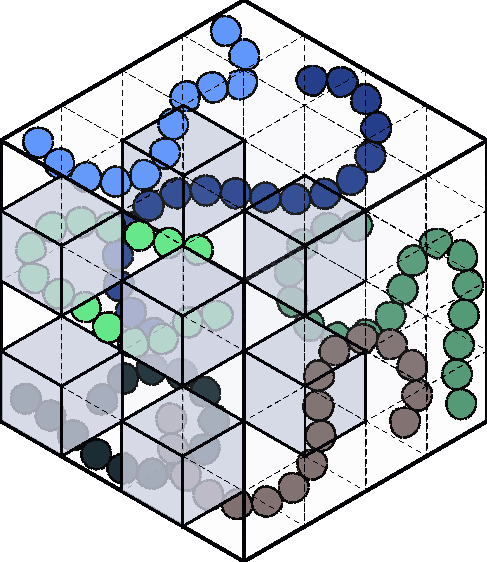
\includegraphics[width=0.95\textwidth]{figs/checkerboard_cube_wpols.pdf}
      \end{minipage}
    };
    }

    \only<5>{
    \node[hilite, below=0.5 of vesicles] (pnesa)
    {
      Effect of model selection on nucleation in polymers\\[2pt] %Self-Assembly\\[3pt]
      \begin{minipage}{.4\textwidth}
      %  \centering
        \raggedright
        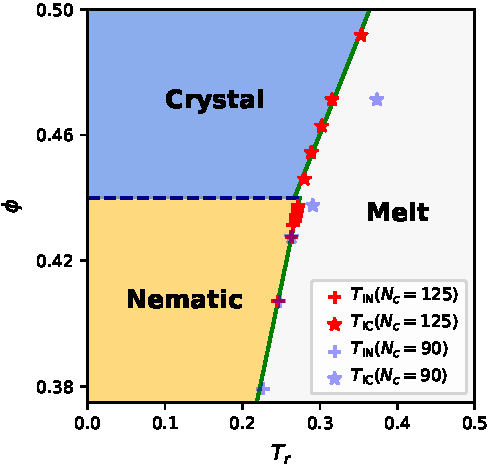
\includegraphics[width=0.95\textwidth]{figs/fig-hard_step_phase_diag.pdf}
      \end{minipage}
      \begin{minipage}{.4\textwidth}
        \raggedleft
        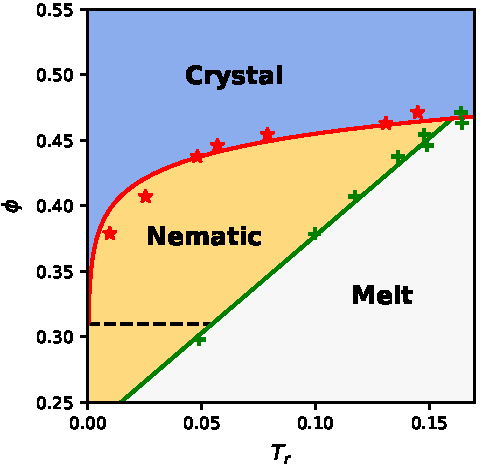
\includegraphics[width=0.95\textwidth]{figs/fig-hard_harm_phase_diag.pdf}
      \end{minipage}

    };
    }

    \node[boxstyle, below=0.5 of vesicles] (pnesa)
    {
      Effect of model selection on nucleation in polymers\\[2pt] %Self-Assembly\\[3pt]
      \begin{minipage}{.4\textwidth}
      %  \centering
        \raggedright
        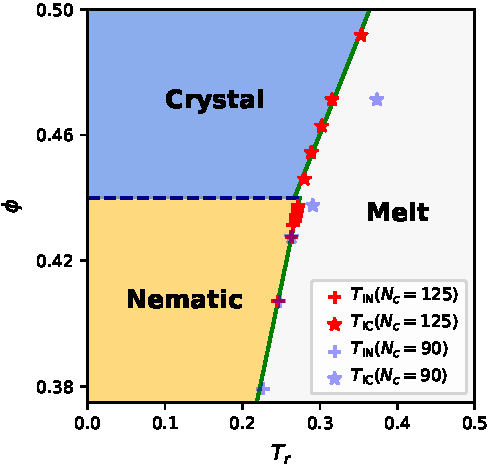
\includegraphics[width=0.95\textwidth]{figs/fig-hard_step_phase_diag.pdf}
      \end{minipage}
      \begin{minipage}{.4\textwidth}
        \raggedleft
        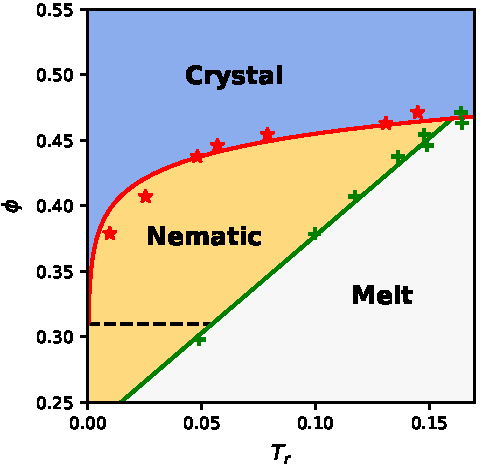
\includegraphics[width=0.95\textwidth]{figs/fig-hard_harm_phase_diag.pdf}
      \end{minipage}

    };

  \end{tikzpicture}

% }}}
\end{frame}

%%\begin{frame}[c]{Melt memory is indicative of unusual crystallization behavior in polymer melts}
%%% {{{
%%% Slide 1: Use Hafele example + other observations slide
%%
%%  \begin{columns}[T]
%%
%%  \column{0.64\textwidth}
%%
%%    \centering
%%%how do I move it to the left
%%    \onslide<1->{
%%    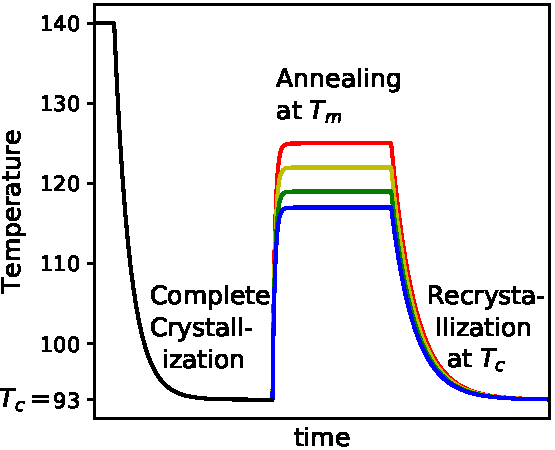
\includegraphics[]{figs/fig-melt_mem.pdf}
%%    }
%%
%%  \column{0.36\textwidth}
%%
%%    \centering
%% %   \hspace{-30pt}
%%    \only<2>{
%%    \vspace{2.0\baselineskip}
%%    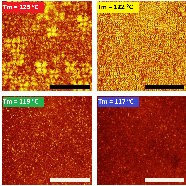
\includegraphics[width=1.1\textwidth]{figs/colored_melt_mem.pdf}
%%    }
%%    
%%    \onslide<3>{
%%    \vspace{1.0\baselineskip}
%%    \begin{block}{Other Observations}
%%      \begin{itemize} 
%%        \item Initial larger scale ordering in SAXS/WAXS measurements
%%        \item Deviant Crystallization and Recrystallization line
%%        \item Intermediate Phase Observations
%%        \item No Copolymer Effect on Crystallization
%%      \end{itemize}
%%    \end{block}
%%    }
%%
%%  \end{columns}
%%%% }}}
%%\end{frame}

%\begin{frame}[t]{The problem: Simulations at equilibrium are difficult and take long times}
%% {{{
%% Slide 0.5 Our approach: - Equilibrium MC sims of polymer crystal CG models.
%\centering
%% }}}
%\end{frame}
%\begin{frame}[c]{How can we simulate polymer crystallization? Different scales}
%% {{{
%  \centering
%  \vspace{2ex}
%  \only<1>{\includegraphics[]{figs/fig-scales_0.pdf}}
%  \only<2>{\includegraphics[]{figs/fig-scales_1.pdf}}
%  \only<3>{\includegraphics[]{figs/fig-scales_1.5.pdf}}
%  \only<4>{\includegraphics[]{figs/fig-scales_2.pdf}}
%  \only<5>{\includegraphics[]{figs/fig-scales_3.pdf}}
%  \only<6>{\includegraphics[]{figs/fig-scales_4.pdf}}
%  \only<7>{\includegraphics[]{figs/fig-scales_5.pdf}}
%
%% }}}
%\end{frame}
%

\begin{frame}[t]{But first, how do we simulate a homopolymer like polyethylene (PE)?}
% {{{
% Slide 0.8: CG models and length scale we study
  \centering

  \includegraphics<1>[width=\textwidth]{../figures/ch1_intro/fig-atom_to_CG_PE/subfig-AA_PE.pdf}

  \includegraphics<2>[width=\textwidth]{../figures/ch1_intro/fig-atom_to_CG_PE/subfig-CG_PE.pdf}

  \only<3>{
    \begin{columns}[T]
    
    \column{0.5\paperwidth}
      \centering
      \vspace{-.2\baselineskip}

      All Atom PE
      \begin{backgroundblock}{0mm}{8.0mm}
        \only<3>{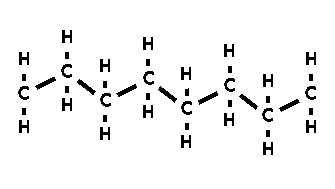
\includegraphics[width=0.95\textwidth]{../figures/ch1_intro/fig-atom_to_CG_PE/subfig-AA_PE.pdf}}
      \end{backgroundblock}

      \vspace{5.6\baselineskip}

      Coarse Grained (CG) PE
      \vspace{-.4\baselineskip}

      \begin{backgroundblock}{0mm}{47mm}
        \only<3>{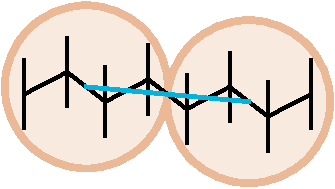
\includegraphics[width=0.95\textwidth]{../figures/ch1_intro/fig-atom_to_CG_PE/subfig-CG_PE.pdf}}
      \end{backgroundblock}

    \column{0.5\paperwidth}
      \centering

      \includegraphics[height=0.9\textheight]{../figures/ch1_intro/fig-atom_to_CG_PE/subfig-long_CG_PE.pdf}

    \end{columns}
  }


% }}}
\end{frame}

\begin{frame}[t]{Specialized moveset moves the polymers from one equilibrium to next}
% {{{
% Slide 0.10: Moveset stuffs
  \centering
%  \includegraphics[height=0.9\textheight]{../figures/ch2_method/fig-polymer_moves/fig-polymer_moves.pdf}
  \begin{columns}[T]
  \column{0.3\textwidth}
    \centering
    \blocktitle{Kink}
    \includegraphics[angle=-90, width=0.6\textwidth]{../figures/ch2_method/fig-polymer_moves/crank_shaft_move.pdf}
  \column{0.3\textwidth}
    \centering
    \blocktitle{End-Kink}
    \includegraphics[angle=-90, width=0.6\textwidth]{../figures/ch2_method/fig-polymer_moves/end_rotation_move.pdf}
  \column{0.3\textwidth}
    \centering
    \blocktitle{Reptation}
    \includegraphics[angle=-90, width=0.6\textwidth]{../figures/ch2_method/fig-polymer_moves/reptation_move.pdf}
  \end{columns}
%TODO add orange stuff and leave only two of em
% }}}
\end{frame}

\begin{frame}[t]{In MC, CG beads move according to potentials and sampling modes}
% {{{
% Slide
  \centering

  \begin{columns}[T]

    \column{0.50\textwidth}
    \centering
    \vspace{-0.5\baselineskip}

    \begin{block}{Molecular simulation inputs}
      \centering

      \begin{itemize}

        \item CG polymer model
        \item Initial positions
        \item Periodic boundary condition
        \item Moveset (kink, end-kink, etc.)
      \end{itemize}

    \end{block}

    %\vspace{0.5\baselineskip}

    \only<2>{
    \begin{block}{More inputs discussed case-by-case}
      \centering

      \begin{itemize}

        \item How beads interact (potential models)
        \item Sampling mode
        \begin{itemize}
          \item Boltzmann for thermodynamic avg
          \item Wand-Landau for entropy
          \item Expanded ensembles for FELs
        \end{itemize}
      \end{itemize}

    \end{block}
    }

    \column{0.45\textwidth}

%    \raggedleft
    \centering
    \includegraphics[height=0.72\textheight]{../figures/fig-initial_config/fig-initial_config.pdf}

  \end{columns}

% }}}
\end{frame}

% Section 1: Domain decomposition of MC
\againframe<3>{outline} % {{{ % }}}
% Slide 1.11: Domain decomposition enables parallel computation

\begin{frame}[t]{Domain decomposition enables parallel computation}
% {{{
% Slide 1.12: Domain decomposition enables parallel computation

  \only<1>{
    \centering
    \vspace{.5\baselineskip}

    \includegraphics[height=0.85\textheight]{figs/just_cube_wdims_wpols.pdf}
  }

  \only<2>{
  \begin{columns}[T]

  \column{0.5\textwidth}
    \centering
    \vspace{-.5\baselineskip}

    \blocktitle{Serial MC}
    \vspace{.5\baselineskip}

    \includegraphics[width=0.85\textwidth]{figs/just_cube_wdims_wpols.pdf}

  \column{0.5\textwidth}
    \centering
    \vspace{-.5\baselineskip}

    \blocktitle{Parallel MC}
    \vspace{.5\baselineskip}

    \includegraphics[width=0.85\textwidth]{figs/checkerboard_cube_wpols.pdf}

  \end{columns}
  }
  
% }}}
\end{frame}

\begin{frame}[t]{Although the parallel algorithm was faster, it was not enough}
% {{{
% Slide 1.13: Domain decomposition enables parallel computation

  \begin{columns}[T]

  \column{0.5\textwidth}
    \centering
    \vspace{.5\baselineskip}
    \includegraphics[]{../figures/ch3_gpu/fig-speedup_new/fig-speedup.pdf}

  \column{0.5\textwidth}

    \centering
    \begin{block}{What we've done}
      Built GPU-accelerated WLMC utilizing
      \begin{itemize} 
      \item Domain and function decomposition
      \item Advanced polymer moveset
    \end{itemize}
    \end{block}

    \begin{block}{What we've learnt}
      \begin{itemize} 
        \item Speedups are modest
        \item Can't simulate large polymers
        \item Focus on small models
        \item Focus on accelerated biased sampling
        \item Build FEL with MC methods
      \end{itemize}
    \end{block}

  \end{columns}
  
%% }}}
\end{frame}

% Section 2: Nucleation mechanisms in a semiflexible oligomer.
\againframe<4>{outline} % {{{ % }}}
% Slide 1.14: Section 2: Nucleation mechanisms in a semiflexible oligomer.

\begin{frame}[c]{We have started with a simple model of semiflexible oligomers}
% {{{
% Slide 2.15: We have started with a simple model of semiflexible oligomers
  \begin{columns}[T]

  \column{0.55\textwidth}

    \centering
    \vspace{-1.0\baselineskip}

      \begin{equation*}
        U_{\mathrm{tot}} = U_{\mathrm{nonbond}}(r_{ij}) + U_{\mathrm{stretch}}(l) + U_{\mathrm{bend}}(\theta)
      \end{equation*}

%      \vspace{0.2\baselineskip}
      \begin{columns}[T, onlytextwidth]

      \column{0.5\textwidth}
   %     \centering
        \vspace{-0.2\baselineskip}

        \onslide<2->{\textcolor{FigGreen}{\Large Hard sphere repulsion}}

      \column{0.5\textwidth}
        \vspace{-1.4\baselineskip}
        \centering

        \onslide<2->{
          \begin{equation*}
            U_{\mathrm{nonbond}} =
            \begin{cases} 
              \infty & r_{\mathrm{ij}} < \sigma \\
              0 & r_{\mathrm{ij}} \ge \sigma
            \end{cases}
          \end{equation*}
        }
      \end{columns}
     
      \vspace{0.6\baselineskip}

      \onslide<3->{
      \begin{columns}[T, onlytextwidth]

      \column{0.5\textwidth}
   %     \centering
        \textcolor{FigOrange}{\Large Rod-like bonds}

      \column{0.5\textwidth}

        \vspace{-1.2\baselineskip}
        \centering
        \begin{equation*}
          U_{\mathrm{stretch}} =
          \begin{cases}
            0 & l = l_{0} \\
            \infty & l \neq l_{0}
          \end{cases}
        \end{equation*}
      \end{columns}
      }

      \vspace{1.3\baselineskip}

      \onslide<4->{
      \begin{columns}[T, onlytextwidth]
      \column{0.5\textwidth}
     %   \centering
        \textcolor{FigPurple}{\Large Stepwise bending stiffness}

      \column{0.5\textwidth}
        \vspace{-1.0\baselineskip}
        \centering

        \begin{equation*}
          U_{\mathrm{bend}} =
          \begin{cases} 
            -k_{b} & \theta \geq \theta_{\mathrm{s}} \\
            0 & \theta < \theta_{\mathrm{s}} 
          \end{cases}
        \end{equation*}
      \end{columns}
      }


      \onslide<5>{
        \vspace{0.2\baselineskip}

        \begin{block}{Phase behavior depends on}
          \begin{itemize}
		  \item Volume Fraction, $\phi = V_{\mathrm{beads}}/V_{\mathrm{box}}$ 
            \item Reduced Temperature, $T_{r} = k_{B}T/k_{b}$
          \end{itemize}
        \end{block}
      }
    %  \only<1>{
    %    \begin{tikzpicture}[remember picture, overlay]
    %        \node[minimum width=14cm, minimum height=4.0cm, fill=white, opacity=1.0] 
    %             at ([xshift=-0.3cm, yshift=-1.8cm] current page.center) {
    %        };

    %    \end{tikzpicture}
    %  }

  \column{0.44\textwidth}

    \centering
    \vspace{\baselineskip}

    \only<2>   {\includegraphics[width=0.95\textwidth]{../figures/fig-hard_tang_step_model/fig-HS_pair_pot.pdf}}
    \only<3>   {\includegraphics[width=0.95\textwidth]{../figures/fig-hard_tang_step_model/fig-tangent_bond.pdf}}
    \only<4>   {\includegraphics[width=0.95\textwidth]{../figures/fig-hard_tang_step_model/fig-stiff_PE.pdf}}
    \only<5>{\includegraphics[width=0.95\textwidth]{../figures/fig-hard_tang_step_model/fig-CG_PE_box_zoom.pdf}}

  \end{columns}
% }}}
\end{frame}

\begin{frame}<1-2>[label=mcfel]{We studied the phase behavior using a combination of MC methods}
% {{{
% Slide 2.16: Overview of what we did

  \begin{tikzpicture}[remember picture, overlay]

    \node[anchor=center, align=center] at (current page.center) {
      \includegraphics[width=0.7\textwidth]{figs/fig-MCFEL_simple.pdf}
    };

    \node[text width=8cm, align=center, anchor=south] at ([yshift=0.1cm] current page.south) {
      \scriptsize{}WLMC:~Wang.~Phys.~Rev.~Lett.~(2001)\par
      \scriptsize{}EXEDOS:~Rathore et al.~J.~Chem.~Phys.~(2004)\par
      \scriptsize{}Kawak, Banks, \& Tree.~J.~Chem.~Phys. (2021)\par
    };

    \only<2>{
    \node[minimum width=10cm, minimum height=3cm, fill=white, opacity=0.7] 
         at ([yshift=-1.5cm] current page.center) {
    };
    }

    \only<3>{
    \node[minimum width=10cm, minimum height=3cm, fill=white, opacity=0.7] 
         at ([yshift=1.5cm] current page.center) {
    };
    }

  \end{tikzpicture}

%Refs for: Wang Landau Monte Carlo (WLMC)
% Wang.~Phys.~Rev.~Lett.~(2001) 
% Taylor et al.~J.~Chem.~Phys.~(2009)
%
%Refs for: Expanded Ensemble Density of States (EXEDOS)
% Rathore et al.~J.~Chem.~Phys.~(2004)
% Chopra et al.~J.~Chem.~Phys.~(2006)
% Shekhar et al.~J.~Chem.~Phys.~(2012)
% Singh et al.~Annu.~Rev.~Chem.~Biomol.~Eng.~(2012)
% Sidky and Whitmer.~Liq.~Cryst.~(2016)

% }}}
\end{frame}

%\begin{frame}[t]{MCMC melting curves.}
%% {{{
%% Slide 2.16 MCMC melting curves.
%\centering
%% }}}
%\end{frame}
%
\begin{frame}[c]{Wang--Landau captures the $T$-dependent thermodynamics at fixed $\phi$}
% {{{
% Slide 2.17: WLMC melting curves.
  \begin{columns}[T]

  \column{0.40\textwidth}
    \centering
    \blocktitle{\centering{}Replica-Exchange WLMC}
    \only<1>{
      \includegraphics[]{figs/fig-WL_DOS_traj.pdf}
    }
    \only<2>{
      \includegraphics[]{figs/fig-WL_DOS_traj_1.pdf}
    }
    \only<3>{
      \includegraphics[]{figs/fig-WL_DOS_traj_2.pdf}
    }
    \only<4->{
      \includegraphics[]{figs/fig-WL_DOS_traj_3.pdf}
    }

  \column{0.40\textwidth}
    \centering
    \onslide<4->{
      \blocktitle{\centering{}Heat Capacity for all $T$}
      \includegraphics[]{figs/fig-WLMC_Cv_plain_10p25.pdf}
    }
  \end{columns}

  \begin{tikzpicture}[remember picture, overlay]

    \onslide<4->{
    \node[] (wlmc) at ([xshift=-0.2cm] current page.center) {};
    \node[] (cv) at ([xshift=0.7cm] current page.center) {};
    \draw[line width=1mm, darkblue, ->] (wlmc) -- (cv);
    }

    %\node[text width=8cm, align=center, anchor=south] at ([yshift=0.1cm] current page.south) {
    %  \scriptsize{}Kawak, Banks, \& Tree.~J.~Chem.~Phys. (2021)\par
    %};
  \end{tikzpicture}

% }}}
\end{frame}

\begin{frame}[c]{Sweeping volume fraction ($\phi$) shows a single first-order phase transition}
% {{{
% Slide 2.18: $\phi$ sweep results.

  \centering
  \vspace{0.3\baselineskip}
  \includegraphics[]{../figures/ch4_jcp/fig-WLMC_all/fig-WLMC_all_Cv.pdf}

  \par

  \begin{tikzpicture}[remember picture, overlay]
    \node[text width=8cm, align=center, anchor=south] at ([yshift=0.1cm] current page.south) {
      \scriptsize{}Kawak, Banks, \& Tree.~J.~Chem.~Phys. (2021)\par
    };
  \end{tikzpicture}

%% }}}
\end{frame}

\begin{frame}[c]{Order parameters reveal two types of transitions}
% {{{
% Slide 2.19: Order parameters reveal two types of transitions}

  \begin{columns}[T, onlytextwidth]
    \column{0.48\textwidth}
      \includegraphics[]{../figures/ch4_jcp/fig-WLMC_all/fig-WLMC_all_Q6.pdf}
    \column{0.48\textwidth}
      \includegraphics[]{../figures/ch4_jcp/fig-WLMC_all/fig-WLMC_all_P2.pdf}
  \end{columns}

  \par

  \begin{tikzpicture}[remember picture, overlay]
    \node[text width=8cm, align=center, anchor=south] at ([yshift=0.1cm] current page.south) {
      \scriptsize{}Kawak, Banks, \& Tree.~J.~Chem.~Phys. (2021)\par
    };
  \end{tikzpicture}


%% }}}
\end{frame}

\begin{frame}[c]{At high $T$ and all $\phi$ the system is an isotropic melt}
% {{{
% Slide 2.20: At high $T$ and all $\phi$ the system is an isotropic melt

  \centering
  \begin{tikzpicture}

    \node[text width=3.5cm, align=center] (a) {
      \includegraphics[width=\textwidth]{figs/fig-melt_OPs.pdf}
    };

    \node[text width=3.5cm, align=center, above=0.0cm of a.south, anchor=north] (b) {
      \includegraphics[width=\textwidth]{figs/melt_struct_yz.pdf}
    };

%    \node[text width=12cm, align=center, above left=1.6cm and -0.0cm of a.east, anchor=north west] (c) {
    \node[text width=8cm, align=center, above left=1.2cm and -0.5cm of a.east, anchor=north west] (c) {
  %    \includegraphics[width=\textwidth]{figs/melt_conf.pdf}
      %\movie[width=8cm, showcontrols, autostart, borderwidth=0pt, loop]{\includegraphics[width=8cm]{../figures/ch2_method/fig-phase_vids/melt.png}}{../figures/ch2_method/fig-phase_vids/melt.mp4}
      \includemovie[text={\includegraphics[width=5.7cm]{../figures/ch2_method/fig-phase_vids/melt.png}}, autoplay=true, mouse=true]{5.7cm}{5.7cm}{../figures/ch2_method/fig-phase_vids/melt.mp4}
      %\includemovie[poster,mouse=true]{8cm}{6cm}{melt.mp4}
    };

  \end{tikzpicture}

  \par\leavevmode

  \begin{tikzpicture}[remember picture, overlay]
    \node[text width=8cm, align=center, anchor=south] at ([yshift=0.1cm] current page.south) {
      \scriptsize{}Kawak, Banks, \& Tree.~J.~Chem.~Phys. (2021)\par
    };
  \end{tikzpicture}

%% }}}
\end{frame}

\begin{frame}[c]{At low $T$ and low $\phi$ the system is nematic}
% {{{
% Slide 2.21: At low $T$ and low $\phi$ the system is nematic

  \centering
  \begin{tikzpicture}

    \node[text width=3.5cm, align=center] (a) {
      \includegraphics[width=\textwidth]{figs/fig-nematic_OPs.pdf}
    };

    \node[text width=3.5cm, align=center, above=0.0cm of a.south, anchor=north] (b) {
      \includegraphics[width=\textwidth]{figs/nematic_struct_xz.pdf}
    };

    \node[text width=8cm, align=center, above left=1.2cm and -0.5cm of a.east, anchor=north west] (c) {
%      \includegraphics[width=\textwidth]{figs/nematic_conf.pdf}
      %\movie[width=8cm, showcontrols, autostart, borderwidth=0pt, loop]{\includegraphics[width=8cm]{../figures/ch2_method/fig-phase_vids/nematic.png}}{../figures/ch2_method/fig-phase_vids/nematic.mp4}
      \includemovie[text={\includegraphics[width=5.7cm]{../figures/ch2_method/fig-phase_vids/nematic.png}}, autoplay=true, mouse=true]{5.7cm}{5.7cm}{../figures/ch2_method/fig-phase_vids/nematic.mp4}
    };
  \end{tikzpicture}

  \leavevmode\par

  \begin{tikzpicture}[remember picture, overlay]
    \node[text width=8cm, align=center, anchor=south] at ([yshift=0.1cm] current page.south) {
      \scriptsize{}Kawak, Banks, \& Tree.~J.~Chem.~Phys. (2021)\par
    };
  \end{tikzpicture}

%% }}}
\end{frame}

\begin{frame}[t]{At low $T$ and high $\phi$ the system is crystalline}
% {{{
% Slide 2.22: At low $T$ and high $\phi$ the system is crystalline

  \centering
  \vspace{-6pt}
  \begin{tikzpicture}

    \node[text width=3.5cm, align=center] (a) {
      \includegraphics[width=\textwidth]{figs/fig-cryst_OPs.pdf}
    };

    \node[text width=3.5cm, align=center, above=0.0cm of a.south, anchor=north] (b) {
      \includegraphics[width=\textwidth]{figs/cryst_struct_yz.pdf}
    };

    \node[text width=8cm, align=center, above left=1.2cm and -0.5cm of a.east, anchor=north west] (c) {
%      \includegraphics[width=\textwidth]{figs/cryst_conf.pdf}
      %\movie[width=8cm, showcontrols, autostart, borderwidth=0pt, loop]{\includegraphics[width=8cm]{../figures/ch2_method/fig-phase_vids/cryst.png}}{../figures/ch2_method/fig-phase_vids/cryst.mp4}
      \includemovie[text={\includegraphics[width=5.7cm]{../figures/ch2_method/fig-phase_vids/cryst.png}}, autoplay=true, mouse=true]{5.7cm}{5.7cm}{../figures/ch2_method/fig-phase_vids/cryst.mp4}
    };

  \end{tikzpicture}

  \leavevmode\par

  \begin{tikzpicture}[remember picture, overlay]
    \node[text width=8cm, align=center, anchor=south] at ([yshift=0.1cm] current page.south) {
      \scriptsize{}Kawak, Banks, \& Tree.~J.~Chem.~Phys. (2021)\par
    };
  \end{tikzpicture}

%% }}}
\end{frame}

\begin{frame}[c]{Melt--nematic--crystal phase diagram}
% {{{
% Slide 2.23: Introduce phase diagram

  \centering
  \vspace{0.2\baselineskip}

  \includegraphics[]{../figures/ch4_jcp/fig-phase_diag/fig-phase_diag.pdf}
%% }}}
\end{frame}

\againframe<3>{mcfel}
% Slide 2.24: Now we move on to FEL analysis

\begin{frame}[c]{To understand interplay of crystal and nematic order, we need 2D FELs}
% {{{
% Slide 2.25: To understand interplay of crystal and nematic order, we need 2D FELs

  \begin{columns}[T]
  
  \column{0.5\textwidth}
    \centering

    \blocktitle{EXEDOS algorithm builds 1D FEL}% \cite{Rathore2004}}
    \includegraphics<1>[]{../figures/fig-EXEDOS_traj/fig-EXEDOS_traj_0.pdf}\includegraphics<2>[]{../figures/fig-EXEDOS_traj/fig-EXEDOS_traj_1.pdf}\includegraphics<3>[]{../figures/fig-EXEDOS_traj/fig-EXEDOS_traj_2.pdf}\includegraphics<4->[]{../figures/fig-EXEDOS_traj/fig-EXEDOS_traj_3.pdf}

  \column{0.5\textwidth}
    \centering

    \only<5->{
    \blocktitle{Our algorithm incorporates 2 OPs}
    \includegraphics[]{../figures/fig-EXEDOS_traj/fig-EXEDOS_2D.pdf}
    }

  \end{columns}
% }}}
\end{frame}

\begin{frame}<1-4>[c]{At low $\phi$, the FEL shows a melt--nematic transition along $P_{2}$}
% {{{
% Slide 2.26: At low $\phi$, the FEL shows a melt--nematic transition along $P_{2}$

  \begin{columns}[T]

  \column{0.65\textwidth}
    \centering
    \includegraphics<1>[]{../figures/fig-pathway_10p75/subfig-pathway_10p75.pdf}\includegraphics<2>[]{../figures/fig-pathway_10p75/fig-pathway_10p75_wConfs.pdf}\includegraphics<3->[]{../figures/fig-pathway_10p75/fig-pathway_10p75_wMFEP.pdf}

  \column{0.35\textwidth}
    \centering
    \includegraphics[]{figs/fig-phase_diag_mark_nematic.pdf}
    \vspace{-0.5\baselineskip}
    \begin{block}{}
      \begin{itemize}
  %       \setlength\itemsep{0.1em}
  %      \item $T_{\mathrm{Isotropic-Nematic}}$ at low $\phi$
        \item Melt at low $P_{2}$
        \item Nematic at high $P_{2}$
        \item<3-> {\color{yellow}{\rule{1cm}{0.1cm}} } Minimum Free Energy Path (MFEP)
        \item<4-> Only $P_{2}$ changes
      \end{itemize}
    \end{block}
    \onslide<3->{{\scriptsize Fu et al.~J.~Chem.~Inf.~Model.~(2020)}}
     
  \end{columns}

  \par\leavevmode

  \only<1>{
    \begin{tikzpicture}[remember picture, overlay]
        \node[minimum width=6cm, minimum height=5.0cm, fill=white, opacity=1.0] 
             at ([xshift=-2.9cm, yshift=-2.7cm] current page.east) {
        };

    \end{tikzpicture}
  }

  \begin{tikzpicture}[remember picture, overlay]
    \node[text width=8cm, align=center, anchor=south west] at ([xshift=+0.3cm, yshift=0.1cm] current page.south) {
      \scriptsize{}Kawak, Banks, \& Tree.~J.~Chem.~Phys. (2021)\par
    };
  \end{tikzpicture}

%% }}}
\end{frame}

%TODO add 10.75 quivers

\begin{frame}<1-4>[c]{At high $\phi$, FEL shows crystallization with cooperative changes in $P_{2}$ \& $Q_{6}$}
% {{{
% Slide 2.27: At high $\phi$, FEL shows shows crystallization with cooperative changes in $P_{2}$ \& $Q_{6}$

  \begin{columns}[T]

  \column{0.65\textwidth}
    \centering
    \includegraphics<1>[]{../figures/fig-pathway_10p25/subfig-pathway_10p25.pdf}\includegraphics<2>[]{../figures/fig-pathway_10p25/fig-pathway_10p25_wConfs.pdf}\includegraphics<3>[]{../figures/fig-pathway_10p25/fig-pathway_10p25_wMFEP.pdf}\includegraphics<4>[]{../figures/fig-pathway_10p25/fig-pathway_10p25_wArrow.pdf}

  \column{0.35\textwidth}
     \centering
     \includegraphics[]{../figures/old_fig-pathway_10p25/fig-phase_diag_mark_cryst.pdf}
     \vspace{-0.5\baselineskip}
     \begin{block}{}
       \begin{itemize}
         \setlength\itemsep{0.5em}
         \item Melt at low $P_{2}$, $Q_{6}$
         \item Crystal at high $P_{2}$, $Q_{6}$
         \item<3-> {\color{yellow}{\rule{1cm}{0.1cm}} } Minimum Free Energy Path (MFEP)
         \item<4>{Cooperative transition}
       \end{itemize}
     \end{block}
     
  \end{columns}

  \leavevmode\par

  \only<1>{
    \begin{tikzpicture}[remember picture, overlay]
        \node[minimum width=6cm, minimum height=5cm, fill=white, opacity=1.0] 
             at ([xshift=-2.9cm, yshift=-2.7cm] current page.east) {
        };

    \end{tikzpicture}
  }


  \begin{tikzpicture}[remember picture, overlay]
    \node[text width=8cm, align=center, anchor=south west] at ([yshift=0.1cm] current page.south) {
      \scriptsize{}Kawak, Banks, \& Tree.~J.~Chem.~Phys. (2021)\par
    };
  \end{tikzpicture}

% }}}
\end{frame}

\begin{frame}[c]{Extracting the barrier height $\Delta F^{\dagger}$ from the MFEP}
% {{{
% Slide 2.28: Extracting the barrier height $\Delta F^{\dagger}$ from the MFEP

  \begin{columns}[T, onlytextwidth]

  \column{0.50\textwidth}

    \centering
    \vspace{-0.5\baselineskip}
   % \includegraphics[width=\textwidth]{../figures/fig-pathway_10p25/fig-pathway_10p25_wMFEP.pdf}
    \includegraphics[width=\textwidth]{figs/subfig-pathway_10p25_small.pdf}

  \column{0.47\textwidth}

    \centering
    \includegraphics[width=\textwidth]{../figures/old_fig-pathway_10p25/subfig-2d_barrier_10p25_small.pdf}

  \end{columns}

  \par 

  \begin{tikzpicture}[remember picture, overlay]
    \node[text width=8cm, align=center, anchor=south] at ([yshift=0.1cm] current page.south) {
      \scriptsize{}Kawak, Banks, \& Tree.~J.~Chem.~Phys. (2021)\par
    };
  \end{tikzpicture}


%% }}}
\end{frame}

\begin{frame}[c]{The barrier height $\Delta F^{\dagger}$ is strong function of $\phi$}
% {{{
% Slide 2.29: The barrier height $\Delta F^{\dagger}$ is strong function of $\phi$

  \centering
  \vspace{0.5\baselineskip}

  \begin{columns}[T]

  \column{0.6\textwidth}
  \includegraphics[]{../figures/ch4_jcp/fig-heights_vs_phi/fig-heights_vs_phi.pdf}

  \column{0.4\textwidth}
    \begin{block}{EXEDOS barrier heights}
    \begin{itemize}
      \setlength\itemsep{.5em}
      \item $t_{\mathrm{order}} \sim \exp \left( \Delta F^{\dagger} \right)$
      \item Enables comparison to experiments and MD
      \item Thermal fluctuations $\sim k_{B}T$
      \item I $\rightarrow$ N is instantaneous
      \item I $\rightarrow$ C has appreciable $t_{\mathrm{order}}$
      \item If $\Delta F^{\dagger} < k_{B}T$, chains undergo I $\rightarrow$ N
    \end{itemize}
    \end{block}

  \end{columns}

  \par\leavevmode

  \begin{tikzpicture}[remember picture, overlay]
    \node[text width=8cm, align=center, anchor=south] at ([yshift=0.1cm] current page.south) {
      \scriptsize{}Kawak, Banks, \& Tree.~J.~Chem.~Phys. (2021)\par
    };
  \end{tikzpicture}

%% }}}
\end{frame}

\begin{frame}<1-2>[c]{Wrapping up: Semiflexible oligomers crystallize in cooperative mechanism}
% {{{
% Slide 2.31: Wrapping up: Semiflexible oligomers crystallize in cooperative mechanism

  \vspace{-1\baselineskip}
  \begin{columns}[T, onlytextwidth]

  \column{0.57\textwidth}

    \centering
    \vspace{0.5\baselineskip}
    \begin{block}{For a system of simple semiflexible oligomers}
      \begin{itemize}
      \item Equilibrium FELs are valuable 
      \item No intermediate between melt and crystal
      \item Nematic and positional ordering \emph{cooperate} in crystallization mechanism
    \end{itemize}
    \end{block}

    {\small{}Kawak, Banks, \& Tree.~J.~Chem.~Phys.~(2021)\par}
  \vspace{0.6\baselineskip}
    \onslide<2>{
    \begin{block}{How general are our conclusions?}
      \begin{itemize} 
        \item Hard step--stiff rods have unique nucleation
        \item More complex intermolecular potentials?
        Bead softness? Continuous stiffness? etc.
      \end{itemize}
    \end{block}
    }

  \column{0.37\textwidth}

  \vspace{0.8\baselineskip}
    \centering
    \includegraphics[]{figs/fig-stiff_PE_single.pdf}

    \vspace{2.5ex}

    \includegraphics[width=\textwidth]{../figures//fig-pathway_10p25/subfig-pathway_10p25_MFEP.pdf}

  \end{columns}
  
% }}}
\end{frame}

% Section 3: Effect of Model selection on phase behavior.
\againframe<5>{outline} % {{{ % }}}
% Slide 3.32: Domain decomposition enables parallel computation

\begin{frame}[t]{How sensitive are our results to the selected model?}
% {{{
% Slide 3.33: How sensitive are our results to the selected model?

  \vspace{-\baselineskip}

  \raggedright
  \begin{fleqn}
  \begin{equation*}
    U_{\mathrm{tot}} = U_{\mathrm{nonbond}}(r_{ij}) \ \ \ \  +  \ \ \ \ U_{\mathrm{stretch}}(l) \ \ \ \ \ \ \ \ \ \ \ \ +  \ \ \ \ \ \ \ \ \ \ \ \ U_{\mathrm{bend}}(\theta)
  \end{equation*}
  \end{fleqn}

  \vspace{-0.5\baselineskip}

  \onslide<2->{
  \begin{columns}[T]

  \column{0.19\textwidth}

    \centering

      \textcolor{FigGreen}{\Large \emph{Hard} spheres}
      \vspace{.5\baselineskip}

      \includegraphics[scale=0.65]{../figures/fig-all_potentials/fig-pairs/fig-pair_hard.pdf}

  \column{0.29\textwidth}

    \centering
      \textcolor{FigOrange}{\Large \emph{Rod} bonds}
      \vspace{1\baselineskip}

      \includegraphics[scale=0.65]{../figures/fig-all_potentials/fig-bonds/fig-bond_rod.pdf}

  \column{0.52\textwidth}

    \centering
      \textcolor{FigPurple}{\Large \emph{Discrete} (stepwise) stiffness}

      \includegraphics[scale=0.65]{../figures/fig-all_potentials/fig-bend/fig-bend_step.pdf}

  \end{columns}

  }

    \vspace{1\baselineskip}

  \onslide<3->{
  \begin{columns}[T]

  \column{0.19\textwidth}
    \centering

    \textcolor{FigGreen}{\Large \emph{Soft} spheres}
    \vspace{1\baselineskip}

    \includegraphics[scale=0.65]{../figures/fig-all_potentials/fig-pairs/fig-pair_soft.pdf}

  \column{0.29\textwidth}
    \centering

    \textcolor{FigOrange}{\Large \emph{Spring} bonds}
    \vspace{1\baselineskip}

    \includegraphics[scale=0.65]{../figures/fig-all_potentials/fig-bonds/fig-bond_spring.pdf}

  \column{0.52\textwidth}
    \centering

    \textcolor{FigPurple}{\Large \emph{Continuous} (harmonic) stiffness}

    \includegraphics[scale=0.65]{../figures/fig-all_potentials/fig-bend/fig-bend_harm.pdf}

  \end{columns}

  }

% }}}
\end{frame}

\begin{frame}[t]{At the same $\phi$, rods with continuous stiffness undergo a 2-step transition}
% {{{
% Slide 3.34: At the same $\phi$, rods with harmonic stiffness experience a 2-step crystallization
  \vspace{.4\baselineskip}

  \centering
  \only<1>{
    \includegraphics[]{../figures/ch5_soft/step_vs_harm/fig-WLMC/fig-WLMC_sep_profs_1.pdf}
  }
  \only<2>{
    \includegraphics[]{../figures/ch5_soft/step_vs_harm/fig-WLMC/fig-WLMC_sep_profs_2.pdf}
  }
  \only<3>{
    \includegraphics[]{../figures/ch5_soft/step_vs_harm/fig-WLMC/fig-WLMC_sep_profs_3.pdf}
  }
  \only<4>{
    \includegraphics[]{../figures/ch5_soft/step_vs_harm/fig-WLMC/fig-WLMC_sep_profs_4.pdf}
  }
% }}}
\end{frame}

\begin{frame}[c]{The melt--nematic--crystal phase diagram strongly depends on stiffness}
% {{{
% Slide 3.35: The melt--nematic--crystal phase diagram depends strongly on the stiffness potential

  \only<1>{
  \begin{columns}[t]

  \column{0.5\textwidth}
    \centering
    \vspace{0.2\baselineskip}

    \blocktitle{Discrete stiffness}
    \includegraphics[scale=0.85]{../figures/ch5_soft/step_vs_harm/fig-phase_diags/from_step/fig-phase_diag.pdf}

  \column{0.5\textwidth}
    \centering
    \vspace{0.2\baselineskip}

    \blocktitle{Continuous stiffness}
    \includegraphics[scale=0.85]{../figures/ch5_soft/step_vs_harm/fig-phase_diags/from_harm/fig-phase_diag.pdf}

  \end{columns}
  }

  \only<2>{
  \begin{columns}[T]

  \column{0.45\textwidth}

    \centering
    \textcolor{FigPurple}{\Large Discrete stiffness}
    \vspace{0.5\baselineskip}

    \includegraphics[scale=0.65]{../figures/fig-all_potentials/fig-bend/fig-bend_step.pdf}

    \vspace{\baselineskip}

    \textcolor{FigPurple}{\Large Continuous stiffness}
    \vspace{0.5\baselineskip}

    \includegraphics[scale=0.65]{../figures/fig-all_potentials/fig-bend/fig-bend_harm.pdf}

  \column{0.55\textwidth}

    \centering
    \vspace{0.5\baselineskip}

    \includegraphics[scale=1.0]{../figures/ch5_soft/step_vs_harm/fig-phase_diags/fig-phase_diag.pdf}
    
  \end{columns}

  }
% }}}
\end{frame}

\begin{frame}[c]{Softness and variable bonds shift the phase boundaries to lower $T$}
% {{{
% Slide 3.36: Softness and variable bonds shift the phase boundaries to lower $T$

  \begin{columns}[T]

  \column{0.45\textwidth}

  \vspace{1.3\baselineskip}

    \begin{columns}[T]

    \column{0.422\textwidth}

      \centering

      \textcolor{FigGreen}{\Large \emph{Hard} spheres}
      \vspace{.5\baselineskip}

      \includegraphics[scale=0.65]{../figures/fig-all_potentials/fig-pairs/fig-pair_hard.pdf}

    \column{0.678\textwidth}

      \centering
      \textcolor{FigOrange}{\Large \emph{Rod} bonds}
      \vspace{.5\baselineskip}

      \includegraphics[scale=0.65]{../figures/fig-all_potentials/fig-bonds/fig-bond_rod.pdf}

    \end{columns}

    \vspace{1.3\baselineskip}

    \begin{columns}[T]

    \column{0.422\textwidth}

      \centering
      \textcolor{FigGreen}{\Large \emph{Soft} spheres}
      \vspace{0.5\baselineskip}

      \includegraphics[scale=0.65]{../figures/fig-all_potentials/fig-pairs/fig-pair_soft.pdf}

    \column{0.678\textwidth}

      \centering
      \textcolor{FigOrange}{\Large \emph{Spring} bonds}
      \vspace{0.5\baselineskip}

      \includegraphics[scale=0.65]{../figures/fig-all_potentials/fig-bonds/fig-bond_spring.pdf}

    \end{columns}

  \column{0.52\textwidth}
    \centering
    \vspace{0.5\baselineskip}

    \includegraphics[]{../figures/ch5_soft/soft_vs_hard/fig-phase_diag.pdf}

  \end{columns}
% }}}
\end{frame}

\begin{frame}[c]{However, comparison of soft and hard beads requires a correction}
% {{{
% Slide 3.37: However, comparison of soft and hard beads requires a correction
  \begin{columns}

  \column{0.39\textwidth}
    \centering
    \vspace{\baselineskip}

    \only<1>{
    \includegraphics[scale=0.9]{../figures/ch5_soft/fig-reff_T/subfig-reff_T.pdf}
    }
    \only<2>{
    \includegraphics[scale=0.9]{../figures/ch5_soft/fig-reff_T/fig-reff_T.pdf}
    }

  \column{0.6\textwidth}
    \centering
    \vspace{\baselineskip}

    \includegraphics<1>[height=0.7\textheight]{../figures/ch5_soft/fig-reff_T/subfig-soft_reff.pdf}
    \includegraphics<2>[scale=0.95]{../figures/ch5_soft/soft_vs_hard/fig-phase_diag_phi_eff.pdf}

  \end{columns}

% }}}
\end{frame}
%
%\begin{frame}[c]{Softness and variable bonds shift the phase boundaries to lower $T$}
%% {{{
%% Slide 3.36: Softness and variable bonds shift the phase boundaries to lower $T$
%  \begin{columns}
%
%  \column{0.5\textwidth}
%    \centering
%    \vspace{0.2\baselineskip}
%
%    \includegraphics[scale=0.85]{../figures/ch5_soft/soft_vs_hard/fig-phase_diag_phi.pdf}
%
%  \column{0.5\textwidth}
%    \centering
%    \vspace{0.2\baselineskip}
%
%    \includegraphics[scale=0.85]{../figures/ch5_soft/soft_vs_hard/fig-phase_diag_phi_eff.pdf}
%
%  \end{columns}
%
%% }}}
%\end{frame}
%
%\begin{frame}<1-2>[c]{Soft beads and continuous stiffness better approximates a real polymer}
%% {{{
%  \begin{columns}[T]
%
%  \column{0.44\textwidth}
%
%    \centering
%    \vspace{-1.0\baselineskip}
%      \onslide<1->{
%      \begin{equation*}
%      U_{tot} = U_{\mathrm{WCA}}(r_{ij}) + U_{\mathrm{bond}}(l) + U_{\mathrm{bend}}(\theta)
%      \end{equation*}
%      \begin{equation*}
%        U_{\mathrm{WCA}} =
%        \begin{cases} 
%          4\epsilon \left[ \frac{\sigma}{r_{ij}}^{12} - \frac{\sigma}{r_{ij}}^6 \right] + \epsilon & r_{\mathrm{ij}} < r_{c} \\
%          0 & r_{\mathrm{ij}} \ge r_{c}
%        \end{cases}
%      \end{equation*}
%      \begin{equation*}
%        U_{bond} = \kappa \left( l - l_{0} \right) ^2
%      \end{equation*}
%      \begin{equation*}
%        U_{bend} = k_{b} \left( 1 - \cos \theta \right)
%      \end{equation*}
%      }
%   %   \includegraphics[scale=0.26]{figs/fig-hard_sphere_rod.pdf}
%
%%    \blocktitle{Classical Nucleation Theory for Polymers}
%%    \includegraphics[]{figs/fig-CNTP_Free_Energy.pdf}
%    \begin{block}{}
%      \begin{itemize} 
%        \item Nematic intermediate (SOMM?)
%        \item Comparison to hard bead chains
%        \item What parameters to explore?
%        \item $l_{b}/\sigma, k_{B}T/k_{b}, \epsilon/k_{b},$ MW
%      \end{itemize}
%    \end{block}
%
%  \column{0.59\textwidth}
%
%      \includegraphics<1>[]{../figures/fig-soft_WLMC_P2_Q6/fig-soft_WLMC_P2_Q6.pdf}
%
%      \includegraphics<2>[]{../figures/fig-phase_diag_soft/fig-phase_diag_soft.pdf}
%
%  \end{columns}
%%% }}}
%\end{frame}

\begin{frame}[t]{Softness and continuous stiffness add a stiffness strength, $k_{b}^{*} = k_{b}/\epsilon$}
% {{{
% Slide 3.38: Effect of bending stiffness.
  \centering
  \begin{columns}

  \column{0.5\textwidth}
    \centering
    \vspace{0.2\baselineskip}

    \includegraphics[]{../figures/ch5_soft/fig-soft_phase_diag_vs_kb/fig-phase_diag_phi_HS.pdf}

  \column{0.5\textwidth}
    \centering
    \vspace{0.2\baselineskip}

    \includegraphics[]{../figures/ch5_soft/fig-soft_phase_diag_vs_kb/fig-phase_diag_phi_eff.pdf}

  \end{columns}
% }}}
\end{frame}

%\begin{frame}<1>[c]{Soft beads and continuous stiffness tells a different story\textcolor{FigPurple}{*}}
%% {{{
%% Slide 3.39: Effect of bending stiffness.
%  \only<1>{
%    \begin{columns}[T]
%
%    \column{0.5\textwidth}
%      \centering
%%      \vspace{-0.5\baselineskip}
%        \blocktitle{At $\phi$, transition after quench\\to below $T_{\mathrm{Isotropic-Nematic}}$}
%        \includegraphics[]{../figures/fig-pathway_soft_nematic/fig-pathway_soft_nematic_wConfs_small.pdf}
%
%    \column{0.5\textwidth}
%      \centering
%%      \vspace{-0.5\baselineskip}
%        \blocktitle{At same $\phi$, further cooling\\leads to $T_{\mathrm{Crystallization}}$}
%        \includegraphics[]{../figures/fig-pathway_soft_cryst/fig-pathway_soft_cryst_wConfs_small.pdf}
%    \end{columns}
%  }
%
%  \begin{tikzpicture}[remember picture, overlay]
%    \node[text width=8cm, align=center, anchor=south east] at ([xshift=-2.0cm,yshift=0.0cm] current page.south) {
%      \small \textcolor{FigPurple}{*\textbf{Preliminary results}}\par
%    };
%  \end{tikzpicture}
%
%%  \onslide<2>{
%%    \begin{columns}[T, onlytextwidth]
%%
%%    \column{0.61\textwidth}
%%    \vspace{1.0\baselineskip}
%%      \begin{columns}[T]
%%        \column{0.5\textwidth}
%%          \centering
%%          \begin{block}{System 1:\\Hard sphere rod chains}
%%            \begin{itemize}
%%              \item Hard sphere
%%              \item Constant bond length
%%              \item Stepwise stiffness
%%              \item No single $\phi$ with both (i.e.\ no intermediate)
%%              \item Neither classical nor SOMM hypothesis
%%            \end{itemize}
%%          \end{block}
%%        \column{0.5\textwidth}
%%          \centering
%%          \begin{block}{System 2:\\Soft bead spring chains}
%%            \begin{itemize}
%%              \item Soft beads
%%              \item Harmonic springs
%%              \item Harmonic stiffness
%%              \item $T_{IN}$ \& $T_{C}$ at same $\phi$
%%              \item SOMM hypothesis applies
%%            \end{itemize}
%%          \end{block}
%%      \end{columns}
%%
%%%      \blocktitle{At $\phi$, transition after quench\\to below $T_{\mathrm{Isotropic-Nematic}}$}
%%      %\includegraphics[width=\textwidth, height=0.4\textheight]{../figures/fig-pathway_soft_nematic/fig-pathway_soft_nematic_wConfs.pdf}
%%    \column{0.35\textwidth}
%%      \includegraphics[]{../figures/fig-pathway_soft_nematic/fig-pathway_soft_nematic_wConfs_smaller.pdf}
%%%      \blocktitle{At same $\phi$, further cooling\\leads to $T_{\mathrm{Crystallization}}$}
%%      \includegraphics[]{../figures/fig-pathway_soft_cryst/fig-pathway_soft_cryst_wConfs_smaller.pdf}
%%  \end{columns}
%%  \leavevmode\par
%%
%%  \begin{tikzpicture}[remember picture, overlay]
%%    \node[text width=8cm, align=center, anchor=south east] at ([xshift=0.5cm,yshift=1.2cm] current page.south) {
%%      \small Kawak, Banks, \& Tree.\ In Preparation (2022)\par
%%    };
%%  \end{tikzpicture}
%%  }
%
%%% }}}
%\end{frame}
%
\begin{frame}[c]{Conclusion: ``This work opens more questions than it answers''}
% {{{
% Slide 3.40: Conclusions!

    \begin{columns}[T, onlytextwidth]

    \column{0.62\textwidth}
      \vspace{-\baselineskip}
      \begin{block}{Polymer models affect nucleation mechanisms}
        \begin{itemize}
            \item Stiffness model selection determines pathways
          \begin{itemize}
            \item Discrete - unique cooperative nucleation
            \item Continuous - more in line with SOMM
          \end{itemize}
          \item Softness and stiffness strength less consequential
          \begin{itemize}
            \item $T_{r}$ corrects for varying stiffness
            \item $\phi_{\mathrm{eff}}$ corrects for varying $T_{m}$
          \end{itemize}
          \item {\small{}Kawak et al.~JCP~(2021)\par}
          \item {\small{}Kawak et al.~(In Prep) \par}
        \end{itemize}
      \end{block}
      \begin{block}{Consequences to polymer theory}
        \begin{itemize} 
          \item Is stiffness more important than connectivity?
          \item Do dihedrals or attraction change conclusions?
        \end{itemize}
      \end{block}

    \column{0.33\textwidth}
      \centering
      \includegraphics[width=139pt]{figs/fig-CNTP_Free_Energy.pdf}
      \includegraphics[width=139pt]{figs/fig-SOMM_Free_Energy.pdf}

  \end{columns}

%% }}}
\end{frame}

\begin{frame}[c]{Conclusions}
% {{{
% Slide 3.41: Conclusions!

  \centering

  \begin{block}{What's next for this research?}
    \begin{itemize} 
      \item What is the effect of more complex potentials? Attraction? Torsional?
      \item Does MD provide similar insights? Compare $t_{\mathrm{order}}$. Thermo versus Kinetics.
      \item FELs of two-step nucleation? Extra dimension of $T_{r}$
    \end{itemize}
  \end{block}
  
  \only<2>{
  \begin{block}{What I've accomplished here at BYU}
    \begin{itemize}
      \item Two open source algorithms for GPU and FEL methods to simulate polymers
      \item One peer-reviewed article {\small{}Kawak et al.~JCP~(2021)} and three more in the works
      \item Presented this work at APS and AIChE annual conferences (2020-2022)
      \item Identified a viable approach to address nucleation mechanisms
      \item Validated the importance of careful model selection to studying crystal nucleation
      \item Cofounded and led the Graduate Student Council in our department
      \item Worked collaboratively with 7 undergraduate researchers
    \end{itemize}
  \end{block}
  }

%% }}}
\end{frame}

\begin{frame}[t]{Acknowledgements}
%% {{{
% Slide 3.42: Acknowledgements

  \centering
  \begin{tikzpicture}
    \node[text width=0.6\columnwidth, align=center, inner sep=0pt, xshift=-0.3] (A) {
    \includegraphics[width=\textwidth]{figs/Tree_Group_Photo_2022.jpg}
    }; 

    \node[text width=0.36\columnwidth, align=center, above left= 3.15cm and -6.0cm of A.east, anchor=north east, inner sep=0pt] (B) {
    \includegraphics[width=\textwidth]{figs/GSC_Group_Photo_2021.jpg}
    }; 

    \node[text width=0.36\columnwidth, align=center, above left= -1.0cm and -6.0cm of A.east, anchor=north east, inner sep=0pt] (C) {
    \includegraphics[width=\textwidth]{figs/Tree_Group_Photo_cake.jpg}
    }; 

  \end{tikzpicture}

  \begin{tikzpicture}[remember picture, overlay]

    \node[inner sep=0pt, align=center, text width=2cm, anchor=south west] at ([yshift=0.3cm, xshift=0.1cm] current page.south west) (A) { 
      \includegraphics[height=1.0cm]{./figs/BYU_IM26b.pdf}
    };

    \node[inner sep=0pt, align=center, right=20 pt of A.east] (D)
    { 
      \includegraphics[height=1.2cm]{./figs/ACS-PRF_logo.jpg}
    };

    \node[inner sep=0pt, align=center, text width=3cm, right = 3 pt of D] (E) { 
      \includegraphics[height=1.0cm]{figs/fig-ORC-logo.pdf}
    };

  \end{tikzpicture}
%% }}}
\end{frame}
%% THE END

%TODO add 10p25 quivers
%TODO decompose 10p25 into delS and delU to make the point
\begin{frame}[t]{Type of transition is determined by interplay of enthalpy and entropy ($\Delta F = \Delta U - T\Delta S$)}
% {{{
% Slide 2.30: The FEL results from an interplay of enthalpic and entropic contributions
  \centering
  \begin{columns}[t]

  \column{0.5\textwidth}
    %\includegraphics<1>[scale=0.8]{../figures/fig-pathway_10p75/subfig-pathway_10p75.pdf}

    \only<1>{\blocktitle{low $\phi$, $\Delta F$}}
    \includegraphics<1>[scale=0.8]{../figures/ch4_jcp/fig-USF/Lx10.75_USF_plots/USF_plot_0.pdf}

    \only<2>{\blocktitle{low $\phi$, $\Delta U$}}
    \includegraphics<2>[scale=0.8]{../figures/ch4_jcp/fig-USF/Lx10.75_USF_plots/USF_plot_1.pdf}

    \only<3>{\blocktitle{low $\phi$, $-T\Delta S$}}
    \includegraphics<3>[scale=0.8]{../figures/ch4_jcp/fig-USF/Lx10.75_USF_plots/USF_plot_2.pdf}

  \column{0.5\textwidth}
    %\includegraphics<1>[scale=0.8]{../figures/fig-pathway_10p25/subfig-pathway_10p25.pdf}

    \only<1>{\blocktitle{high $\phi$, $\Delta F$}}
    \includegraphics<1>[scale=0.8]{../figures/ch4_jcp/fig-USF/Lx10.00_USF_plots/USF_plot_0.pdf}

    \only<2>{\blocktitle{high $\phi$, $\Delta U$}}
    \includegraphics<2>[scale=0.8]{../figures/ch4_jcp/fig-USF/Lx10.00_USF_plots/USF_plot_1.pdf}

    \only<3>{\blocktitle{high $\phi$, $-T\Delta S$}}
    \includegraphics<3>[scale=0.8]{../figures/ch4_jcp/fig-USF/Lx10.00_USF_plots/USF_plot_2.pdf}

  \end{columns}

%TODO fix figures into low and high panel for low and high phi
% }}}
\end{frame}


% CUDA Extra Notes
\begin{frame}[t]{Regular serial MC}
% {{{
% Slide 1.07 Regular serial MC
  \vspace{-1ex}
  \begin{columns}[T]
  \column{0.5\textwidth}
    \centering
%    \blocktitle{}
    \begin{block}{}
      \begin{algorithm}[H]
      \caption{Basic MC algorithm}\label{alg:cap}
      \begin{algorithmic}[1]
\State $R \gets $read\_conf()
\State $E \gets $calc\_energy($R$)
\For{\texttt{$i < num\_moves$}}
  \color{red}\State $R_{\mathrm{new}} \gets $do\_move()
  \color{black}\State $E_{\mathrm{new}} \gets $calc\_energy($R_{\mathrm{new}}$)
  \State $P_{\mathrm{acc}} \gets $exp($-\beta(E_{\mathrm{new}}-E)$)
  \If{$P_{\mathrm{acc}} > $ rand(0,1)} 
%    \Comment{Accept with $P_{\mathrm{acc}}$}
    \State $E \gets E_{\mathrm{new}}$
    \State $R \gets R_{\mathrm{new}}$
  \EndIf
\EndFor

\end{algorithmic}
\end{algorithm}
    \end{block}
  \column{0.5\textwidth}
    \onslide<2->{
    \centering
%    \blocktitle{End-bridging}
    \includegraphics[width=\textwidth, trim=0 2 270 0, clip]{figs/DomainDecomp.png}
    }
  \end{columns}

  \onslide<3>{
  \begin{tikzpicture}[remember picture, overlay]

    \node[fill=white, minimum width=6cm, minimum height=2cm, 
          rounded corners=0.2cm, anchor=center, opacity=0.7] 
          at (current page.center) {
    };

    \node[text width=5cm, fill=lightblue, draw=darkblue, very thick, rounded corners=0.2cm, anchor=center] 
          at (current page.center) {
      How can we "GPU-accelerate"\\inherently serial code?
    };

  \end{tikzpicture}
  }
  
% }}}
\end{frame}

\begin{frame}[c]{Checkerboarding our domain makes MC massively parallel}
% Slide 1.13 Domain decomposition of MC
% {{{

  \vspace{-1ex}
  \begin{columns}[T]
  \column{0.5\textwidth}
    \centering
    \blocktitle{Boring MC}
    \includegraphics[width=\textwidth, trim=0 2 270 0, clip]{figs/DomainDecomp.png}
  \column{0.5\textwidth}
    \centering
    \blocktitle{Checkerboard MC}
    \includegraphics[width=\textwidth, trim=270 2 0 0, clip]{figs/DomainDecomp.png}
    \vspace{0.7\baselineskip}
    \scriptsize Anderson et al.~J.~Comp.~Phys. (2013)
  \end{columns}
  
% }}}
\end{frame}

\begin{frame}[c]{Polymer-specific moveset improves sampling further}
% {{{

  \vspace{-1ex}
  \begin{columns}[T]
  \column{0.44\textwidth}
    \centering
    \blocktitle{Configurational bias}
    \includegraphics[width=\textwidth]{figs/config_bias_move.pdf}
  \column{0.28\textwidth}
    \onslide<2,3>{
    \centering
    \blocktitle{End-bridging}
    \includegraphics[width=\textwidth]{figs/end_bridge_move.pdf}
    }
  \column{0.28\textwidth}
    \onslide<3>{
    \centering
    \blocktitle{Double-bridging}
    \includegraphics[width=\textwidth]{figs/dbl_bridge_move.pdf}
    }
  \end{columns}
% }}}
\end{frame}

\begin{frame}[c]{Our code speeds up polymer simulations by 2 orders of magnitude!!!}
% {{{
% Slide 1.15 Speedup.

  \begin{columns}[T]
  \column{0.5\textwidth}
    \centering
    \includegraphics[]{figs/fig-accuracy.pdf}
  \column{0.5\textwidth}
    \centering
    \includegraphics[]{figs/fig-speedup.pdf}
  \end{columns}

% }}}
\end{frame}

\begin{frame}[c]{Despite overcoming slow equilibration, the system spanned too many orders of magnitude to be solved in reasonable time}
% {{{

  \begin{columns}[t]
  \column{0.5\textwidth}
    \centering
    %\includegraphics[width=\textwidth, trim=205 10 215 80, clip]{figs/fig-title_page_conf.png}
    \begin{overpic}[width=\textwidth, trim=205 10 215 80, clip]{figs/fig-title_page_conf.png}
      \put (0,90) {\noindent\colorbox{black} {\color{white}\huge 2000 Chain} }
      \put (0,80) {\noindent\colorbox{black} {\color{white}\huge 100 Bead Melt} }
    \end{overpic}
  \column{0.5\textwidth}
    \centering
    \begin{overpic}[]{figs/fig-duration_bar.pdf}
      \only<2->{
        \put (22,10) {\noindent\colorbox{black} {\color{white}\huge Crystalline} }
      }
      \only<3->{
        \put (0,67) {\noindent\colorbox{violet} {\color{white}\Large Shakirov \& Paul simulated 720x10} }
        \put (0,60) {\noindent\colorbox{violet} {\color{white}\Large Their system spanned 5,600 OoM!} }
        \put (5,53) {\noindent\colorbox{violet} {\color{white}\Large Ours spans 200,000 OoM!} }
        \put (5,46) {\noindent\colorbox{violet} {\color{white}\normalsize Shakirov \& Paul.~Phys.~Rev.~E (2018)} }
      }
    \end{overpic}
  \end{columns}
% }}}
\end{frame}

\begin{frame}[c]{Conclusions}
% {{{
% Slide 1.16 Conclusions & future work

  \begin{columns}[T, onlytextwidth]

  \column{0.57\textwidth}

    \centering
    \begin{block}{What we've done}
      Built GPU-accelerated WLMC utilizing
      \begin{itemize} 
      \item Domain and function decomposition
      \item Advanced polymer moveset
    \end{itemize}
    \end{block}

    \begin{block}{What we've learnt}
      \begin{itemize} 
        \item Problem: Too many OoM
        \item Should investigate order parameter response (potentials of mean force)
        \item Focus on specific temperature 
      \end{itemize}
    \end{block}

    \vspace{4pt}
    \begin{tikzpicture}

      \node[inner sep=0pt, align=center ] (A)
      { 
        \includegraphics[height=1.0cm]{./figs/BYU_IM26b.pdf}
      };

      \node[inner sep=0pt, align=center, anchor=center, right=9 pt of A.east] (B)
      { 
        \includegraphics[height=1.2cm]{./figs/ACS-PRF_logo.jpg}
      };

      \node[inner sep=0pt, align=center, text width=3cm, right = 3 pt of B] (C) { 
        \includegraphics[height=1.0cm]{figs/fig-ORC-logo.pdf}
      };

    \end{tikzpicture}

  \column{0.37\textwidth}

    \centering
    \includegraphics[width=\textwidth]{figs/fig-speedup_small.pdf}

    \vspace{8pt}
    \begin{tikzpicture}

      \node[inner sep=0pt, align=center, text width=2cm] (D) { 
        \includegraphics[height=2.0cm]{figs/Douglas.jpeg}
      };

      \node[inner sep=0pt, align=center, text width=2cm, right= 0 pt of D.east, anchor=west] (E) { 
        \includegraphics[height=2.0cm]{figs/Dakota.pdf}
      };

    \end{tikzpicture}


  \end{columns}
  
%% }}}
\end{frame}

\begin{frame}[c]{At low $\phi$, the FEL shows a melt--nematic transition along $P_{2}$}
% {{{

  \begin{columns}[T]

  \column{0.5\textwidth}
    \centering
    \includegraphics[width=\textwidth]{../figures/fig-pathway_10p75/subfig-pathway_10p75.pdf}

  \column{0.5\textwidth}
    \centering
    \includegraphics[width=\textwidth]{../figures/ch4_jcp/fig-quivers_10p75/fig-quiver_10.75.pdf}
     
  \end{columns}

%% }}}
\end{frame}

\begin{frame}[c]{At low $\phi$, the FEL shows a melt--nematic transition along $P_{2}$}
% {{{

  \begin{columns}[T]

  \column{0.5\textwidth}
    \centering
    \includegraphics[width=\textwidth]{../figures/ch4_jcp/fig-quivers_10p75/fig-U_quiver_10.75.pdf}

  \column{0.5\textwidth}
    \centering
    \includegraphics[width=\textwidth]{../figures/ch4_jcp/fig-quivers_10p75/fig-mTS_quiver_10.75.pdf}
     
  \end{columns}

%% }}}
\end{frame}

\begin{frame}[c]{At high $\phi$, FEL shows crystallization with cooperative changes in $P_{2}$ \& $Q_{6}$}
% {{{

  \begin{columns}[T]

  \column{0.5\textwidth}
    \centering
    \includegraphics[width=\textwidth]{../figures/fig-pathway_10p25/subfig-pathway_10p25.pdf}

  \column{0.5\textwidth}
    \centering
    \includegraphics[width=\textwidth]{../figures/ch4_jcp/fig-quivers_10p25/fig-quiver_10p25.pdf}
     
  \end{columns}

% }}}
\end{frame}

\begin{frame}[c]{At high $\phi$, FEL shows crystallization with cooperative changes in $P_{2}$ \& $Q_{6}$}
% {{{

  \begin{columns}[T]

  \column{0.5\textwidth}
    \centering
    \includegraphics[width=\textwidth]{../figures/ch4_jcp/fig-quivers_10p25/fig-U_quiver_10p25.pdf}

  \column{0.5\textwidth}
    \centering
    \includegraphics[width=\textwidth]{../figures/ch4_jcp/fig-quivers_10p25/fig-mTS_quiver_10p25.pdf}
     
  \end{columns}

% }}}
\end{frame}

\begin{frame}[c]{}
% {{{

  \centering
  \includegraphics[height=\textheight]{../figures/ch1_intro/fig-CNT_Free_Energy_wConfs/fig-CNT_Free_Energy_wConfs_v2.pdf}

% }}}
\end{frame}

\begin{frame}[c]{}
% {{{

  \centering
  \includegraphics[width=\textwidth]{../figures/ch1_intro/fig-atom_to_CG_PE/fig-atom_to_CG_PE.pdf}

% }}}
\end{frame}

\begin{frame}[c]{}
% {{{

  \centering
  \includegraphics[height=\textheight]{../figures/ch2_method/fig-potentials/fig-potentials.pdf}

% }}}
\end{frame}

\begin{frame}[c]{}
% {{{

  \centering
    \includegraphics[width=\textwidth]{../figures/ch2_method/fig-acf/fig-acf.pdf}

% }}}
\end{frame}

\begin{frame}[c]{}
% {{{

  \centering
    \includegraphics[height=\textheight]{../figures/ch2_method/fig-phase_confs/fig-phase_confs.pdf}

% }}}
\end{frame}

\begin{frame}[c]{}
% {{{

  \centering
    \includegraphics[height=\textheight]{../figures/ch2_method/fig-UandCv/fig-UandCv.pdf}

% }}}
\end{frame}

\begin{frame}[c]{}
% {{{

  \centering
    \includegraphics[height=\textheight]{../figures/ch2_method/fig-polymer_sizes/fig-polymer_sizes.pdf}

% }}}
\end{frame}

\begin{frame}[c]{}
% {{{

  \centering
  \includegraphics[height=\textheight]{../figures/ch3_gpu/fig-domain_decomp_types/fig-domain_decomp_types.pdf}

% }}}
\end{frame}

\begin{frame}[c]{}
% {{{

  \centering
  \includegraphics[width=\textwidth]{../figures/ch3_gpu/fig-domain_decomp_moves/fig-domain_decomp_moves.pdf}

% }}}
\end{frame}

\begin{frame}[c]{}
% {{{

  \centering
  \includegraphics[height=\textheight]{../figures/ch3_gpu/fig-accuracy/fig-accuracy.pdf}

% }}}
\end{frame}

\begin{frame}[c]{}
% {{{

  \centering
  \includegraphics[height=\textheight]{../figures/ch3_gpu/fig-Fytas_MC_WL_replicate/fig-Fytas_MC_WL_replicate}

% }}}
\end{frame}

\begin{frame}[c]{}
% {{{

  \centering
  \includegraphics[height=\textheight]{../figures/ch3_gpu/fig-speedup/fig-speedup.pdf}

% }}}
\end{frame}

\begin{frame}[c]{}
% {{{

  \centering
  \includegraphics[height=\textheight]{../figures/ch3_gpu/fig-speedup_ratios/fig-speedup.pdf}

% }}}
\end{frame}

\begin{frame}[c]{}
% {{{

  \centering
  \includegraphics[height=\textheight]{../figures/ch3_gpu/fig-speedup_efficiency/fig-speedup.pdf}

% }}}
\end{frame}

\begin{frame}[c]{}
% {{{

  \centering
  \includegraphics[width=\textwidth]{../figures/ch3_gpu/fig-CPU_vs_GPU_arch/fig-CPU_vs_GPU_arch.pdf}

% }}}
\end{frame}

\begin{frame}[c]{}
% {{{

  \centering
  \includegraphics[height=\textheight]{../figures/ch3_gpu/fig-GPU_arch/fig-GPU_arch.pdf}

% }}}
\end{frame}

\begin{frame}[c]{}
% {{{

  \centering
  \includegraphics[height=\textheight]{../figures/ch4_jcp_from_diss/fig-pathway_ToC_chains/fig-pathway_ToC_chains.pdf}

% }}}
\end{frame}

\begin{frame}[c]{}
% {{{

  \centering
  \includegraphics[height=\textheight]{../figures/ch4_jcp_from_diss/fig-MCFEL_toolkit_connections/fig-MCFEL_toolkit_connections_V3.pdf}

% }}}
\end{frame}

\begin{frame}[c]{}
% {{{

  \centering
  \includegraphics[height=\textheight]{../figures/ch4_jcp_from_diss/fig-lp_vs_T/fig-lp_vs_T.pdf}

% }}}
\end{frame}

\begin{frame}[c]{}
% {{{

  \centering
  \includegraphics[height=\textheight]{{../figures/ch4_jcp_from_diss/fig-WLMC_plus_MCMC_10.25/fig-WLMC_plus_MCMC_10.25}.pdf}

% }}}
\end{frame}

\begin{frame}[c]{}
% {{{

  \centering
  \includegraphics[height=\textheight]{../figures/ch4_jcp_from_diss/fig-WLMC_all/fig-WLMC_all.pdf}

% }}}
\end{frame}

\begin{frame}[c]{}
% {{{

  \centering
  \includegraphics[height=\textheight]{../figures/ch4_jcp_from_diss/fig-confs_plus_structs/fig-confs_plus_structs.pdf}

% }}}
\end{frame}

\begin{frame}[c]{}
% {{{

  \centering
  \includegraphics[height=\textheight]{../figures/ch4_jcp_from_diss/fig-phase_diag/fig-phase_diag.pdf}

% }}}
\end{frame}

\begin{frame}[c]{}
% {{{

  \centering
  \includegraphics[height=\textheight]{../figures/ch4_jcp_from_diss/fig-FELs_all/fig-FELs_all.pdf}

% }}}
\end{frame}

\begin{frame}[c]{}
% {{{

  \centering
  \includegraphics[height=\textheight]{{../figures/ch4_jcp_from_diss/fig-pathway_10.25/fig-pathway_10.25}.pdf}

% }}}
\end{frame}

\begin{frame}[c]{}
% {{{

  \centering
  \includegraphics[height=\textheight]{../figures/ch4_jcp_from_diss/fig-heights_vs_phi/fig-heights_vs_phi.pdf}

% }}}
\end{frame}

\begin{frame}[c]{}
% {{{

  \centering
  \includegraphics[height=\textheight]{{../figures/ch4_jcp_from_diss/fig-WLMC_plus_MCMC_10.00/fig-WLMC_plus_MCMC_10.0}.pdf}

% }}}
\end{frame}

\begin{frame}[c]{}
% {{{

  \centering
  \includegraphics[height=\textheight]{{../figures/ch4_jcp_from_diss/fig-WLMC_plus_MCMC_10.33/fig-WLMC_plus_MCMC_10.33}.pdf}

% }}}
\end{frame}

\begin{frame}[c]{}
% {{{

  \centering
  \includegraphics[height=\textheight]{{../figures/ch4_jcp_from_diss/fig-WLMC_plus_MCMC_10.50/fig-WLMC_plus_MCMC_10.5}.pdf}

% }}}
\end{frame}

\begin{frame}[c]{}
% {{{

  \centering
  \includegraphics[height=\textheight]{{../figures/ch4_jcp_from_diss/fig-WLMC_plus_MCMC_10.75/fig-WLMC_plus_MCMC_10.75}.pdf}

% }}}
\end{frame}

\begin{frame}[c]{}
% {{{

  \centering
  \includegraphics[height=\textheight]{{../figures/ch4_jcp_from_diss/fig-pathway_10.00/fig-pathway_10.0}.pdf}

% }}}
\end{frame}

\begin{frame}[c]{}
% {{{

  \centering
  \includegraphics[height=\textheight]{{../figures/ch4_jcp_from_diss/fig-pathway_10.33/fig-pathway_10.33}.pdf}

% }}}
\end{frame}

\begin{frame}[c]{}
% {{{

  \centering
  \includegraphics[height=\textheight]{{../figures/ch4_jcp_from_diss/fig-pathway_10.50/fig-pathway_10.5}.pdf}

% }}}
\end{frame}

\begin{frame}[c]{}
% {{{

  \centering
  \includegraphics[height=\textheight]{{../figures/ch4_jcp_from_diss/fig-pathway_10.75/fig-pathway_10.75}.pdf}

% }}}
\end{frame}

\begin{frame}[c]{}
% {{{

  \centering
  \includegraphics[height=\textheight]{../figures/ch5_soft_from_diss/fig-WCA_vs_harmStretch/fig-WCA_vs_harmStretch.pdf}

% }}}
\end{frame}

\begin{frame}[c]{}
% {{{

  \centering
  \includegraphics[height=\textheight]{../figures/ch5_soft_from_diss/fig-all_lp_vs_T/fig-lp_vs_T.pdf}

% }}}
\end{frame}

\begin{frame}[c]{}
% {{{

  \centering
  \includegraphics[height=\textheight]{../figures/ch5_soft_from_diss/figs-hard_step/fig-WLMC_side_phi/fig-WLMC.pdf}

% }}}
\end{frame}

\begin{frame}[c]{}
% {{{

  \centering
  \includegraphics[height=\textheight]{../figures/ch5_soft_from_diss/figs-hard_step/fig-phase_diag_Nc/fig-phase_diag.pdf}

% }}}
\end{frame}

\begin{frame}[c]{}
% {{{

  \centering
  \includegraphics[height=\textheight]{../figures/ch5_soft_from_diss/figs-hard_harm/fig-WLMC_side_phi/fig-WLMC.pdf}

% }}}
\end{frame}

\begin{frame}[c]{}
% {{{

  \centering
  \includegraphics[height=\textheight]{../figures/ch5_soft_from_diss/figs-hard_harm/fig-phase_diag/fig-phase_diag.pdf}

% }}}
\end{frame}

\begin{frame}[c]{}
% {{{

  \centering
  \includegraphics[height=\textheight]{../figures/ch5_soft_from_diss/fig-harm_vs_step_phase_diag/fig-phase_diag.pdf}

% }}}
\end{frame}

\begin{frame}[c]{}
% {{{

  \centering
  \includegraphics[width=\textwidth]{../figures/ch5_soft_from_diss/fig-softxhard_harm_phase_diag/fig-phase_diag.pdf}

% }}}
\end{frame}

\begin{frame}[c]{}
% {{{

  \centering
  \includegraphics[width=\textwidth]{../figures/ch5_soft_from_diss/figs-soft_harm_harm/fig-phase_diag_all/fig-phase_diag_phiHS.pdf}

% }}}
\end{frame}

\begin{frame}[t]{Thank you for not being stereotypical!}
%% {{{
% Slide 3.42: Acknowledgements

  \centering
  \begin{tikzpicture}
    \node[text width=0.7\columnwidth, align=center, inner sep=0pt] (A) {
    \includegraphics[width=\textwidth]{figs/committee_meme.png}
    }; 

  \end{tikzpicture}

%% }}}
\end{frame}

\begin{frame}{Monte Carlo (MC) simulations can simulate material phase behavior}
% {{{
% Slide 0.9:  What are MC sims?
  \centering
  \includegraphics[]{figs/fig-MC_alg_inputs_outputs.pdf}
%TODO maybe add images
%}}}
\end{frame}

\begin{frame}{Monte Carlo simulations can simulate material phase behavior}
% {{{
% Slide 0.9:  What are MC sims?
  \centering
  \only<1>{
    \includegraphics[width=\textwidth]{figs/fig-CG_MolSim_1.pdf}
  }
  
  \only<2>{
    \includegraphics[width=\textwidth]{figs/fig-CG_MolSim_2.pdf}
  }
  
  \only<3>{
    \includegraphics[width=\textwidth]{figs/fig-CG_MolSim_3.pdf}
  }
  
  \only<4>{
    \includegraphics[width=\textwidth]{figs/fig-CG_MolSim_4.pdf}
  }
  
  \only<5>{
    \includegraphics[width=\textwidth]{figs/fig-CG_MolSim.pdf}
  }
% }}
\end{frame}


\end{document}
